\documentclass[lang=cn,math=mtpro2,11pt,scheme=chinese]{elegantbook}

\title{考研数学真题错题整理}
\subtitle{参考 2026 版《考研数学这十年》}

\author{Guangchen Jiang}
% \institute{Elegant\LaTeX{} Program}
\date{2025/12/31}
\version{4.5}
% \bioinfo{自定义}{信息}

% \extrainfo{注意:本模板自 2023 年 1 月 1 日开始,不再更新和维护!}

\setcounter{tocdepth}{3}

\logo{logo-blue.png}
\cover{cover.jpg}

% 本文档命令
\usepackage{array}
\usepackage{amsmath}   % 用于 \pmatrix 矩阵环境
\usepackage{tasks}     % 用于水平排列选项
\usepackage{xifthen} 
\usepackage{pifont}
\usepackage{nicefrac}
% \usepackage{ifthen}       % 确保 \ifthenelse 命令可用
% \usepackage{pifont}       % 确保 \ding 命令可用 (用于图标)
% \usepackage{tcolorbox}    % 确保 tcolorbox 可用
\usepackage{graphicx}
\usepackage{fontawesome5}  % 用于提供图标,例如 \faPencil
% 加载 tcolorbox 的 "skins" 和 "theorems" 库
\tcbuselibrary{skins, theorems}  % 用于处理 \problem 命令的可选参数
\newcommand{\ccr}[1]{\makecell{{\color{#1}\rule{1cm}{1cm}}}}

% 修改标题页的橙色带
\definecolor{customcolor}{RGB}{32,178,170}
\colorlet{coverlinecolor}{customcolor}
\usepackage{cprotect}

\makeatother % 恢复@的原始含义

% 定义题目计数器
\newcounter{problemcounter}[section]

\renewcommand{\problem}[2][]{
  \par\medskip\noindent 
  %
  % --- 下面的代码不变 ---
  \stepcounter{problemcounter}% 计数器加 1 (第一题变1, 第二题变2...)
  \arabic{problemcounter}.% 打印题号 1.
  \ifthenelse{\isempty{#1}}{}{ 【#1】}% 打印可选信息 (25-2)
  \space % 打印一个空格
  #2 % 打印题目正文
}
\renewcommand{\proofname}{答案}
\renewcommand{\notename}{注}

\newcommand{\probtagged}[2][]{%
  \par\noindent%
  % 左侧小图标
  \makebox[0pt][r]{%
    \scriptsize\color{orange!90}\faExclamationTriangle\quad%
  }%
  % 正文部分
  \stepcounter{problemcounter}%
  \arabic{problemcounter}.%
  \ifthenelse{\isempty{#1}}{}{ 【#1】}%
  \space #2%
  \par%
}

% (可选) 全局设置 tasks 环境的样式
% 这里我们设置为4列,标签格式为 A. B. C. ...
\settasks{
  counter-format = (\Alph*), % 标签格式为 A. B. ...
  label-width = 2em,         % 标签宽度
  item-indent = 3em,         % 选项内容缩进
}
\newcommand{\ansat}[1]{%
  \par\nobreak % <--- 关键解决方案:结束上文,并禁止在此处分页
  \vspace{0.3em} % 在 proof 环境前添加您想要的间距
  \begin{proof}
    P#1
  \end{proof}
  \vspace{5em} % <--- 修正:在 proof 环境后添加一些间距 (例如 0.5em)
}

\makeatletter
\newcommand{\rmnum}[1]{\romannumeral #1}
\newcommand{\Rmnum}[1]{\expandafter\@slowromancap\romannumeral #1@}
\makeatother

% \usepackage{setspace} 
% \setstretch{1.3}

\addbibresource[location=local]{reference.bib} % 参考文献,不要删除

\begin{document}

\maketitle
\frontmatter

\tableofcontents

\mainmatter

\chapter{高数}

\section{极限}
% --- 题目 ---
\problem[P2-1 (24-2)]{已知数列 $\displaystyle \{a_n\}$ ($\displaystyle a_n \neq 0$). 若 $\displaystyle \{a_n\}$ 发散, 则 ( \quad )}
\begin{tasks}(2)
  \task $\displaystyle \left\{a_n + \frac{1}{a_n}\right\}$ 发散.
  \task $\displaystyle \left\{a_n - \frac{1}{a_n}\right\}$ 发散.
  \task $\displaystyle \left\{\mathrm{e}^{a_n} + \frac{1}{\mathrm{e}^{a_n}}\right\}$ 发散.
  \task $\displaystyle \left\{\mathrm{e}^{a_n} - \frac{1}{\mathrm{e}^{a_n}}\right\}$ 发散.
\end{tasks}
\ansat{238;【十年真题】 - 考点:极限的概念与性质 - 1}

% --- 题目 ---
\problem[P2-2 (22-1,2)]{设数列 $\displaystyle \{x_n\}$ 满足 $\displaystyle -\frac{\pi}{2} \leqslant x_n \leqslant \frac{\pi}{2}$, 则 ( \quad )}
\begin{tasks}(1)
  \task 当 $\displaystyle \lim_{n \to \infty} \cos(\sin x_n)$ 存在时, $\lim_{n \to \infty} x_n$ 存在.
  \task 当 $\displaystyle \lim_{n \to \infty} \sin(\cos x_n)$ 存在时, $\lim_{n \to \infty} x_n$ 存在.
  \task 当 $\displaystyle \lim_{n \to \infty} \cos(\sin x_n)$ 存在时, $\lim_{n \to \infty} \sin x_n$ 存在, 但 $\lim_{n \to \infty} x_n$ 不一定存在.
  \task 当 $\displaystyle \lim_{n \to \infty} \sin(\cos x_n)$ 存在时, $\lim_{n \to \infty} \cos x_n$ 存在, 但 $\displaystyle \lim_{n \to \infty} x_n$ 不一定存在.
\end{tasks}
\ansat{238;【十年真题】 - 考点:极限的概念与性质 - 2}

% --- 题目 ---
\problem[P4-4 (99-2)]{对任意给定的 $\displaystyle \varepsilon \in (0, 1)$,总存在正整数 $\displaystyle N$,当 $\displaystyle n \ge N$ 时,恒有 $\displaystyle |x_n - a| \le 2\varepsilon$" 是数列 $\displaystyle \{x_n\}$ 收敛于 $\displaystyle a$ 的 ( \quad )}
\begin{tasks}(2)
  \task 充分条件但非必要条件.
  \task 必要条件但非充分条件.
  \task 充分必要条件.
  \task 既非充分条件又非必要条件.
\end{tasks}
\ansat{238;【真题精选】 - 考点:极限的概念与性质 - 4}

% --- 题目 ---
\problem[P4-2 (23-3)]{$\displaystyle \lim_{x \to \infty} x^2 \left(2 - x \sin \frac{1}{x} - \cos \frac{1}{x}\right) = \underline{\hspace{3em}}.$}
\ansat{238;【十年真题】 - 考点一:函数极限的计算 - 2}

% --- 题目 ---
\problem[P4-3 (22-2,3)]{$\displaystyle \lim_{x \to 0} \left(\frac{1+\mathrm{e}^x}{2}\right)^{\cot x} = \underline{\hspace{3em}}.$}
\ansat{238;【十年真题】 - 考点一:函数极限的计算 - 3}

% --- 题目 ---
\problem[P4-7 (16-2,3)]{求极限 $\displaystyle \lim_{x \to 0} (\cos 2x + 2x \sin x)^{\frac{1}{x^4}}$.}
\ansat{239;【十年真题】 - 考点一:函数极限的计算 - 7}

% --- 题目 ---
\problem[P4-2 (25-2)]{$\displaystyle \lim_{n \to \infty} \frac{1}{n^2} \left[ \ln \frac{1}{n} + 2\ln \frac{2}{n} + \dots + (n-1)\ln \frac{n-1}{n} \right] = \underline{\hspace{3em}}.$}
\ansat{239;【十年真题】 - 考点二:数列极限的计算 - 2}

% --- 题目 ---
\problem[P4-5 (19-1,3)]{设 $\displaystyle a_n = \int_{0}^{1} x^n \sqrt{1 - x^2} \mathrm{d}x \ (n = 0, 1, 2, \dots)$.}
\begin{enumerate}
\item[(1)] 证明: 数列 $\displaystyle \{a_n\}$ 单调减少, 且 $\displaystyle a_n = \frac{n-1}{n+2} a_{n-2} \ (n=2, 3, \dots)$;
\item[(2)] 求 $\displaystyle \lim_{n \to \infty} \frac{a_n}{a_{n-1}}$.
\end{enumerate}
\ansat{239;【十年真题】 - 考点二:数列极限的计算 - 5}

% --- 题目 ---
\problem[P4-6 (18-1,2,3)]{设数列 $\displaystyle \{x_n\}$ 满足:$\displaystyle x_1 > 0, \ x_n \mathrm{e}^{x_{n+1}} = \mathrm{e}^{x_n} - 1 \ (n = 1, 2, \dots)$. 证明 $\displaystyle \{x_n\}$ 收敛, 并求 $\displaystyle \lim_{n \to \infty} x_n$.}
\ansat{240;【十年真题】 - 考点二:数列极限的计算 - 6}

% --- 题目 ---
\problem[P6-例1 (2)]{$\displaystyle \lim_{x \to 0} \frac{\sqrt{1+x} - \sqrt{1+\tan x}}{x \tan^2 x} = \underline{\hspace{3em}}.$}
\ansat{6;【方法探究】 - 考点一:函数极限的计算 - 例1 (2)}

% --- 题目 ---
\problem[P7-变式 1.1 (97-2)]{求极限 $\displaystyle \lim_{x \to -\infty} \frac{\sqrt{4x^2+x-1}+x+1}{\sqrt{x^2+\sin x}}$.}
\ansat{240;【方法探究】 - 考点一:函数极限的计算 - 变式 1.1}

% --- 题目 ---
\problem[P8-变式 3 (98-1)]{求极限 $$\lim_{n \to \infty} \left( \frac{\sin \frac{\pi}{n}}{n+1} + \frac{\sin \frac{2\pi}{n}}{n + \frac{1}{2}} + \dots + \frac{\sin \pi}{n + \frac{1}{n}} \right).$$}
\ansat{240;【方法探究】 - 考点二:数列极限的计算 - 变式 3}

% --- 题目 ---
\probtagged[P8-变式 4.1 (96-1)]{设 $\displaystyle x_1 = 10, \ x_{n+1} = \sqrt{6+x_n} \ (n = 1, 2, \dots)$. 试证数列 $\displaystyle \{x_n\}$ 极限存在, 并求此极限.}
\ansat{241;【方法探究】 - 考点二:数列极限的计算 - 变式 4.1}

% --- 题目 ---
\problem[P8-变式 4.2 (11-1, 2)]{(1) 证明:对任意的正整数 $\displaystyle n$, 都有 $\displaystyle \frac{1}{n+1} < \ln\left(1+\frac{1}{n}\right) < \frac{1}{n}$ 成立;
\newline
(2) 设 $\displaystyle a_n = 1 + \frac{1}{2} + \dots + \frac{1}{n} - \ln n (n = 1, 2, \dots)$, 证明数列 $\displaystyle \{a_n\}$ 收敛.}
\begin{note}
  主要错的是 (2)
\end{note}
\ansat{241;【方法探究】 - 考点二:数列极限的计算 - 变式 4.2}
\vspace{2em}

\section{一元函数微分学}
% --- 题目 ---
\problem[P18-1 (25-2)]{设函数 $\displaystyle f(x)$ 连续, 给出下列四个条件:
\\
\textcircled{1} $\displaystyle \lim_{x \to 0} \frac{|f(x)| - f(0)}{x}$ 存在;
\\
\textcircled{2} $\displaystyle \lim_{x \to 0} \frac{f(x) - f(0)}{x}$ 存在;
\\
\textcircled{3} $\displaystyle \lim_{x \to 0} \frac{|f(x)|}{x}$ 存在;
\\
\textcircled{4} $\displaystyle \lim_{x \to 0} \frac{|f(x)| - |f(0)|}{x}$ 存在.
\\
其中能得到 “$\displaystyle f(x)$ 在 $\displaystyle x=0$ 处可导” 的条件的个数是~(~\quad~)
\begin{tasks}(4)
\task 1.
\task 2.
\task 3.
\task 4.
\end{tasks}}
\ansat{249;【十年真题】 - 考点:导数与微分的概念 - 1}

% --- 题目 ---
\problem[P18-7 (16-1)]{已知函数 $\displaystyle f(x) = \begin{cases} \displaystyle x, & \displaystyle x \le 0, \\ \displaystyle \frac{1}{n}, & \displaystyle \frac{1}{n+1} < x \le \frac{1}{n}, n = 1, 2, \dots, \end{cases}$ 则~(~\quad~)}
\begin{tasks}(2)
\task $\displaystyle x=0$ 是 $\displaystyle f(x)$ 的第一类间断点.
\task $\displaystyle x=0$ 是 $\displaystyle f(x)$ 的第二类间断点.
\task $\displaystyle f(x)$ 在 $\displaystyle x=0$ 处连续但不可导.
\task $\displaystyle f(x)$ 在 $\displaystyle x=0$ 处可导.
\end{tasks}
\ansat{250;【十年真题】 - 考点:导数与微分的概念 - 7}

% --- 题目 ---
\problem[P18-8 (25-2,3)]{设函数 $\displaystyle f(x)$ 在 $\displaystyle x = 0$ 处连续, 且 $\displaystyle \lim_{x \to 0} \frac{x f(x) - \mathrm{e}^{2\sin x} + 1}{\ln(1+x) + \ln(1-x)} = -3$, 证明 $\displaystyle f(x)$ 在 $\displaystyle x=0$ 处可导, 并求 $\displaystyle f'(0)$.}
\ansat{250;【十年真题】 - 考点:导数与微分的概念 - 8}

% --- 题目 ---
\problem[P18-9 (22-2)]{已知函数 $\displaystyle f(x)$ 在 $\displaystyle x=1$ 处可导, 且 $$\displaystyle \lim_{x \to 0} \frac{f(\mathrm{e}^{x^2}) - 3f(1 + \sin^2 x)}{x^2} = 2,$$ 求 $\displaystyle f^{\prime}(1)$.}
\ansat{250;【十年真题】 - 考点:导数与微分的概念 - 9}

% --- 题目 ---
\problem[P20-1 (07-1,2,3)]{设函数 $\displaystyle f(x)$ 在 $\displaystyle x=0$ 处连续, 下列命题错误的是~(~\quad~)
\begin{tasks}(2)
\task 若 $\displaystyle \lim_{x \to 0} \frac{f(x)}{x}$ 存在, 则 $\displaystyle f(0)=0$.
\task 若 $\displaystyle \lim_{x \to 0} \frac{f(x)+f(-x)}{x}$ 存在, 则 $\displaystyle f(0)=0$.
\task 若 $\displaystyle \lim_{x \to 0} \frac{f(x)}{x}$ 存在, 则 $\displaystyle f'(0)$ 存在.
\task 若 $\displaystyle \lim_{x \to 0} \frac{f(x)-f(-x)}{x}$ 存在, 则 $\displaystyle f'(0)$ 存在.
\end{tasks}}
\ansat{250;【真题精选】 - 考点:导数与微分的概念 - 1}

% --- 题目 ---
\problem[P20-3 (05-1,2)]{设函数 $\displaystyle f(x) = \lim_{n \to \infty} \sqrt[n]{1+|x|^{3n}}$, 则 $\displaystyle f(x)$ 在 $\displaystyle (-\infty, +\infty)$ 内~(~\quad~)}
\begin{tasks}(2)
\task 处处可导.
\task 恰有一个不可导点.
\task 恰有两个不可导点.
\task 至少有三个不可导点.
\end{tasks}
\ansat{251;【真题精选】 - 考点:导数与微分的概念 - 3}

% --- 题目 ---
\problem[P21-9 (03-3)]{设函数 $\displaystyle f(x) = \begin{cases} \displaystyle x^\lambda \cos \frac{1}{x}, & \displaystyle x \neq 0, \\ \displaystyle 0, & \displaystyle x=0, \end{cases}$ 其导函数在 $\displaystyle x=0$ 处连续, 则 $\displaystyle \lambda$ 的取值范围是 \underline{\hspace{4em}}.}
\ansat{251;【真题精选】 - 考点:导数与微分的概念 - 9}

% --- 题目 ---
\problem[P21-2 (22-2)]{已知函数 $\displaystyle y=y(x)$ 由方程
\[ x^2 + xy + y^3 = 3 \]
确定, 则 $\displaystyle y''(1) = \underline{\hspace{4em}}. $}
\ansat{251;【十年真题】 - 考点一:函数的求导与微分法则 - 2}
\vspace{12em}

% --- 题目 ---
\problem[P21-1 (21-1)]{设函数 $\displaystyle f(x)=\frac{\sin x}{1+x^2}$ 在 $\displaystyle x=0$ 处的 3 次泰勒多项式为 $\displaystyle ax+bx^2+cx^3$, 则~(~\quad~)}
\begin{tasks}(2)
\task $\displaystyle a=1, b=0, c=-\frac{7}{6}$.
\task $\displaystyle a=1, b=0, c=\frac{7}{6}$.
\task $\displaystyle a=-1, b=-1, c=-\frac{7}{6}$.
\task $\displaystyle a=-1, b=-1, c=\frac{7}{6}$.
\end{tasks}
\ansat{251;【十年真题】 - 考点二:高阶导数的计算 - 1}

% --- 题目 ---
\problem[P21-7 (16-1)]{设函数 $\displaystyle f(x) = \arctan x - \frac{x}{1+ax^2}$, 且 $\displaystyle f'''(0) = 1$, 则 $\displaystyle a = \underline{\hspace{4em}}. $}
\ansat{251;【十年真题】 - 考点二:高阶导数的计算 - 7}

% --- 题目 ---
\problem[P24-例(2)]{设函数 $\displaystyle y=x^2 \sin 2x$, 则 $\displaystyle y^{(5)}(0) = \underline{\hspace{4em}}. $}
\ansat{24;【方法探究】 - 考点二:高阶导数的计算 - 例(2)}

% --- 题目 ---
\problem[P25-7 (97-3)]{设 $\displaystyle y = f(\ln x) \mathrm{e}^{f(x)}$, 其中 $\displaystyle f$ 可微, 则 $\displaystyle \mathrm{d}y = \underline{\hspace{4em}}. $}
\ansat{252;【真题精选】 - 考点一:函数的求导与微分法则 - 7}

% --- 题目 ---
\problem[P26-2 (20-3)]{曲线 $\displaystyle x + y + \mathrm{e}^{2xy} = 0$ 在点 $\displaystyle (0, -1)$ 处的切线方程为 $\underline{\hspace{4em}}.$}
\ansat{254;【十年真题】 - 考点一:平面曲线的切线与法线 - 2}

% --- 题目 ---
\problem[P26-1 (23-2)]{设函数 $\displaystyle f(x)=(x^2+a)\mathrm{e}^x$. 若 $f(x)$ 没有极值点, 但曲线 $y=f(x)$ 有拐点, 则 $a$ 的取值范围是~(~\quad~)}
\begin{tasks}(4)
  \task $\displaystyle [0,1).$
  \task $\displaystyle [1, +\infty).$
  \task $\displaystyle [1, 2)$
  \task $\displaystyle [2, +\infty).$
\end{tasks}
\ansat{254;【十年真题】 - 考点二:利用导数判断函数的性质 - 1}

% --- 题目 ---
\problem[P26-2 (22-2)]{设函数 $\displaystyle f(x)$ 在 $\displaystyle x=x_0$ 处具有 2 阶导数, 则~(~\quad~)}
\begin{tasks}(1)
  \task 当 $\displaystyle f(x)$ 在 $\displaystyle x_0$ 的某邻域内单调增加时, $\displaystyle f'(x_0)>0$.
  \task 当 $\displaystyle f'(x_0)>0$ 时, $\displaystyle f(x)$ 在 $\displaystyle x_0$ 的某邻域内单调增加.
  \task 当 $\displaystyle f(x)$ 在 $\displaystyle x_0$ 的某邻域内是凹函数时, $\displaystyle f''(x_0)>0$.
  \task 当 $\displaystyle f''(x_0)>0$ 时, $\displaystyle f(x)$ 在 $\displaystyle x_0$ 的某邻域内是凹函数.
\end{tasks}
\ansat{254;【十年真题】 - 考点二:利用导数判断函数的性质 - 2}

% --- 题目 ---
\problem[P26-4 (19-1)]{设函数 $\displaystyle f(x)=\begin{cases} x|x|, & x \le 0, \\ x\ln x, & x > 0, \end{cases}$ 则 $\displaystyle x=0$ 是 $\displaystyle f(x)$ 的~(~\quad~)}
\begin{tasks}(2)
  \task 可导点, 极值点.
  \task 不可导点, 极值点.
  \task 可导点, 非极值点.
  \task 不可导点, 非极值点.
\end{tasks}
\ansat{254;【十年真题】 - 考点二:利用导数判断函数的性质 - 4}

% --- 题目 ---
\problem[P26-5 (16-2,3)]{设函数 $\displaystyle f(x)$ 在 $\displaystyle (-\infty, +\infty)$ 内连续, 其导函数的图形如下图所示, 则~(~\quad~)
\begin{center}
    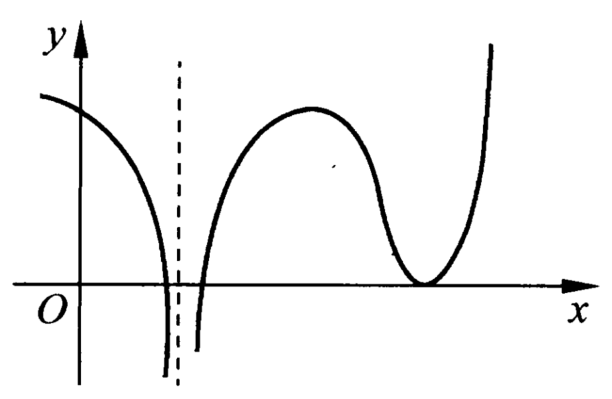
\includegraphics[width=0.5\textwidth]{P26-5_16-2_3.png} % 
\end{center}
\begin{tasks}(1)
  \task 函数 $\displaystyle f(x)$ 有 2 个极值点, 曲线 $\displaystyle y=f(x)$ 有 2 个拐点.
  \task 函数 $\displaystyle f(x)$ 有 2 个极值点, 曲线 $\displaystyle y=f(x)$ 有 3 个拐点.
  \task 函数 $\displaystyle f(x)$ 有 3 个极值点, 曲线 $\displaystyle y=f(x)$ 有 1 个拐点.
  \task 函数 $\displaystyle f(x)$ 有 3 个极值点, 曲线 $\displaystyle y=f(x)$ 有 2 个拐点.
\end{tasks}}
\ansat{254;【十年真题】 - 考点二:利用导数判断函数的性质 - 5}

% --- 题目 ---
\problem[P26-6 (19-2,3)]{曲线 $\displaystyle y = x \sin x + 2 \cos x \ \left(-\frac{\pi}{2} < x < \frac{3\pi}{2}\right)$ 的拐点坐标为 $\underline{\hspace{4em}}.$}
\ansat{254;【十年真题】 - 考点二:利用导数判断函数的性质 - 6}

% --- 题目 ---
\problem[P26-9 (21-2)]{已知函数 $\displaystyle f(x) = \frac{x|x|}{1+x}$, 求曲线 $\displaystyle y=f(x)$ 的凹凸区间及渐近线.}
\ansat{254;【十年真题】 - 考点二:利用导数判断函数的性质 - 9}

% --- 题目 ---
\problem[P27-1 (18-3)]{设某产品的成本函数 $\displaystyle C(Q)$ 可导, 其中 $\displaystyle Q$ 为产量. 若产量为 $\displaystyle Q_0$ 时平均成本最小, 则~(~\quad~)}
\begin{tasks}(2)
  \task $\displaystyle C'(Q_0)=0$.
  \task $\displaystyle C'(Q_0)=C(Q_0)$.
  \task $\displaystyle C'(Q_0)=Q_0 C(Q_0)$.
  \task $\displaystyle Q_0 C'(Q_0)=C(Q_0)$.
\end{tasks}
\ansat{256;【十年真题】 - 考点五:导数的经济应用(仅数学三) - 1}

\vspace{2em}

\section{一元函数积分学}

\section{微分方程}

\section{多元函数微分学}

\section{多元函数积分学}

\section{无穷级数}

\chapter{线代}

\section{行列式}
% --- 题目 ---
\problem[P146-4 (20-1,2,3)]{行列式 $\displaystyle \begin{vmatrix} a & 0 & -1 & 1 \\ 0 & a & 1 & -1 \\ -1 & 1 & a & 0 \\ 1 & -1 & 0 & a \end{vmatrix} = \underline{\hspace{4em}}.$}
\ansat{323;【十年真题】 - 考点:具体行列式的计算 - 4}

% --- 题目 ---
\problem[P148-例2 (1)]{$\displaystyle n$ 阶行列式 $\displaystyle \begin{vmatrix} 1 & -1 & & & & \\ 2 & a & -1 & & & \\ 3 & & a & -1 & & \\ \vdots & & \ddots & \ddots & & \\ n-1 & & & & a & -1 \\ n & & & & & a \end{vmatrix} = \underline{\hspace{4em}}.$}
\ansat{148;【方法探究】 - 考点:具体行列式的计算 - 例2 (1)}

% --- 题目 ---
\problem[P149-4 (96-5)]{5 阶行列式 $\displaystyle \begin{vmatrix} 1-a & a & 0 & 0 & 0 \\ -1 & 1-a & a & 0 & 0 \\ 0 & -1 & 1-a & a & 0 \\ 0 & 0 & -1 & 1-a & a \\ 0 & 0 & 0 & -1 & 1-a \end{vmatrix} = \underline{\hspace{4em}}.$}
\ansat{324;【真题精选】 - 考点:具体行列式的计算 - 4}


\vspace{2em}

\section{矩阵}
% --- 题目 ---
\problem[P150-3 (24-1)]{设实矩阵 $\displaystyle \bm{A} = \begin{pmatrix} a+1 & a \\ a & a \end{pmatrix}$. 若对任意实向量 $\displaystyle \boldsymbol{\alpha} = \begin{pmatrix} x_1 \\ x_2 \end{pmatrix}, \ \boldsymbol{\beta} = \begin{pmatrix} y_1 \\ y_2 \end{pmatrix}$, 
$$\displaystyle (\boldsymbol{\alpha}^{\mathrm{T}} \bm{A} \boldsymbol{\beta})^2 \le \boldsymbol{\alpha}^{\mathrm{T}} \bm{A} \boldsymbol{\alpha} \cdot \boldsymbol{\beta}^{\mathrm{T}} \bm{A} \boldsymbol{\beta}$$ 
都成立, 则 $\displaystyle a$ 的取值范围为 \underline{\hspace{4em}}.}
\ansat{325;【十年真题】 - 考点一:矩阵的运算 - 3}

% --- 题目 ---
\problem[P150-4 (22-1)]{已知矩阵 $\displaystyle \bm{A}$ 和 $\displaystyle \bm{E}-\bm{A}$ 可逆, 其中 $\displaystyle \bm{E}$ 为单位矩阵. 若矩阵 $\displaystyle \bm{B}$ 满足 $\displaystyle [\bm{E} - (\bm{E} - \bm{A})^{-1}]\bm{B} = \bm{A}$, 则 $\displaystyle \bm{B} - \bm{A} = \underline{\hspace{4em}}. $}
\ansat{325;【十年真题】 - 考点一:矩阵的运算 - 4}

% --- 题目 ---
\problem[P150-1 (25-2)]{下列矩阵中, 可以经过若干初等行变换得到矩阵 $\displaystyle \begin{pmatrix} 1 & 1 & 0 & 1 \\ 0 & 0 & 1 & 2 \\ 0 & 0 & 0 & 0 \end{pmatrix}$ 的是~(~\quad~)}
\begin{tasks}(4)
  \task $\displaystyle \begin{pmatrix} 1 & 1 & 0 & 1 \\ 1 & 2 & 1 & 3 \\ 2 & 3 & 1 & 4 \end{pmatrix}.$
  \task $\displaystyle \begin{pmatrix} 1 & 1 & 0 & 1 \\ 1 & 1 & 2 & 5 \\ 1 & 1 & 1 & 3 \end{pmatrix}.$
  \task $\displaystyle \begin{pmatrix} 1 & 0 & 0 & 1 \\ 0 & 1 & 0 & 3 \\ 0 & 1 & 0 & 0 \end{pmatrix}.$
  \task $\displaystyle \begin{pmatrix} 1 & 1 & 2 & 3 \\ 1 & 2 & 2 & 3 \\ 2 & 3 & 4 & 6 \end{pmatrix}.$
\end{tasks}
\ansat{325;【十年真题】 - 考点二:矩阵的初等变换与初等矩阵 - 1}

% --- 题目 ---
\problem[P150-4 (22-2,3)]{设 $\displaystyle \bm{A}$ 为 3 阶矩阵, 交换 $\displaystyle \bm{A}$ 的第 2 行和第 3 行, 再将第 2 列的 $\displaystyle -1$ 倍加到第 1 列, 得到 $\displaystyle \begin{pmatrix} -2 & 1 & -1 \\ 1 & -1 & 0 \\ -1 & 0 & 0 \end{pmatrix}$, 则 $\displaystyle \bm{A}^{-1}$ 的迹 $\displaystyle \mathrm{tr}(\bm{A}^{-1}) = \underline{\hspace{4em}}.$}
\ansat{325;【十年真题】 - 考点二:矩阵的初等变换与初等矩阵 - 4}
\vspace{4em}

% --- 题目 ---
\problem[P150-2 (24-2)]{设 $\displaystyle \bm{A}$ 为 4 阶矩阵, $\displaystyle \bm{A}^*$ 为 $\displaystyle \bm{A}$ 的伴随矩阵. 若 $\displaystyle \bm{A}(\bm{A} - \bm{A}^*) = \bm{O}$, 且 $\displaystyle \bm{A} \neq \bm{A}^*$, 则 $\displaystyle r(\bm{A})$ 取值为~(~\quad~)}
\begin{tasks}(4)
  \task $\displaystyle 0$ 或 $\displaystyle 1$.
  \task $\displaystyle 1$ 或 $\displaystyle 3$.
  \task $\displaystyle 2$ 或 $\displaystyle 3$.
  \task $\displaystyle 1$ 或 $\displaystyle 2$.
\end{tasks}
\ansat{325;【十年真题】 - 考点三:矩阵的秩与等价 - 2}

% --- 题目 ---
\problem[P156-10 (95-1)]{设 $\displaystyle \bm{A}$ 是 $\displaystyle n$ 阶矩阵, 满足 $\displaystyle \bm{A}\bm{A}^{\mathrm{T}}=\bm{E}$ ($\displaystyle \bm{E}$ 是 $\displaystyle n$ 阶单位矩阵, $\displaystyle \bm{A}^{\mathrm{T}}$ 是 $\displaystyle \bm{A}$ 的转置矩阵), $\displaystyle |\bm{A}| < 0$, 则 $\displaystyle |\bm{A} + \bm{E}| = \underline{\hspace{4em}}. $}
\ansat{327;【真题精选】 - 考点一:矩阵的运算 - 10}

% --- 题目 ---
\problem[P156-3 (01-3)]{设}
\[ \bm{A} = \begin{pmatrix} a_{11} & a_{12} & a_{13} & a_{14} \\ a_{21} & a_{22} & a_{23} & a_{24} \\ a_{31} & a_{32} & a_{33} & a_{34} \\ a_{41} & a_{42} & a_{43} & a_{44} \end{pmatrix}, \bm{B} = \begin{pmatrix} a_{14} & a_{13} & a_{12} & a_{11} \\ a_{24} & a_{23} & a_{22} & a_{21} \\ a_{34} & a_{33} & a_{32} & a_{31} \\ a_{44} & a_{43} & a_{42} & a_{41} \end{pmatrix}, \]
\[ \bm{P}_1 = \begin{pmatrix} 0 & 0 & 0 & 1 \\ 0 & 1 & 0 & 0 \\ 0 & 0 & 1 & 0 \\ 1 & 0 & 0 & 0 \end{pmatrix}, \bm{P}_2 = \begin{pmatrix} 1 & 0 & 0 & 0 \\ 0 & 0 & 1 & 0 \\ 0 & 1 & 0 & 0 \\ 0 & 0 & 0 & 1 \end{pmatrix}, \]
$\displaystyle \bm{A}$ 可逆, 则 $\displaystyle \bm{B}^{-1} =~(~\quad~)$
\begin{tasks}(4)
  \task $\displaystyle \bm{A}^{-1}\bm{P}_1\bm{P}_2.$
  \task $\displaystyle \bm{P}_1\bm{A}^{-1}\bm{P}_2.$
  \task $\displaystyle \bm{P}_1\bm{P}_2\bm{A}^{-1}.$
  \task $\displaystyle \bm{P}_2\bm{A}^{-1}\bm{P}_1.$
\end{tasks}
\ansat{327;【真题精选】 - 考点二:矩阵的初等变换与初等矩阵 - 3}

% --- 题目 ---
\problem[P156-5 (08-1)]{设 $\displaystyle \boldsymbol{\alpha}, \boldsymbol{\beta}$ 为 3 维列向量, 矩阵 $\displaystyle \bm{A} = \boldsymbol{\alpha}\boldsymbol{\alpha}^{\mathrm{T}} + \boldsymbol{\beta}\boldsymbol{\beta}^{\mathrm{T}}$, 其中 $\displaystyle \boldsymbol{\alpha}^{\mathrm{T}}$ 为 $\displaystyle \boldsymbol{\alpha}$ 的转置, $\displaystyle \boldsymbol{\beta}^{\mathrm{T}}$ 为 $\displaystyle \boldsymbol{\beta}$ 的转置. 证明:}
\begin{enumerate}
\item[(1)] $\displaystyle r(\bm{A}) \le 2$;
\item[(2)] 若 $\displaystyle \boldsymbol{\alpha}, \boldsymbol{\beta}$ 线性相关, 则 $\displaystyle r(\bm{A}) < 2$.
\end{enumerate}
\ansat{327;【真题精选】 - 考点三:矩阵的秩与等价 - 5}

\vspace{2em}

\section{向量与线性方程组}
% --- 题目 ---
\problem[P158-5 (23-2,3)]{已知线性方程组}
\[ \begin{cases} ax_1 + x_3 = 1, \\ x_1 + ax_2 + x_3 = 0, \\ x_1 + 2x_2 + ax_3 = 0, \\ ax_1 + bx_2 = 2 \end{cases} \]
{有解, 其中 $\displaystyle a, b$ 为常数. 若 $\displaystyle \begin{vmatrix} a & 0 & 1 \\ 1 & a & 1 \\ 1 & 2 & a \end{vmatrix} = 4$, 则 $\displaystyle \begin{vmatrix} 1 & a & 1 \\ 1 & 2 & a \\ a & b & 0 \end{vmatrix} = \underline{\hspace{4em}}. $}
\ansat{328;【十年真题】 - 考点一:线性方程组的解的情况及求解 - 5}

% --- 题目 ---
\problem[P159-1 (18-1,2,3)]{已知 $\displaystyle a$ 是常数, 且矩阵 $\displaystyle \bm{A} = \begin{pmatrix} 1 & 2 & a \\ 1 & 3 & 0 \\ 2 & 7 & -a \end{pmatrix}$ 可经初等列变换化为矩阵 $\displaystyle \bm{B} = \begin{pmatrix} 1 & a & 2 \\ 0 & 1 & 1 \\ -1 & 1 & 1 \end{pmatrix}.$}
\begin{enumerate}
\item[(1)] 求 $\displaystyle a$;
\item[(2)] 求满足 $\displaystyle \bm{AP} = \bm{B}$ 的可逆矩阵 $\displaystyle \bm{P}$.
\end{enumerate}
\ansat{328;【十年真题】 - 考点二:矩阵方程组的解的情况及求解 - 1}
\vspace{8em}

% --- 题目 ---
\problem[P159-2 (16-1)]{设矩阵
\[ \bm{A} = \begin{pmatrix} 1 & -1 & -1 \\ 2 & a & 1 \\ -1 & 1 & a \end{pmatrix}, \bm{B} = \begin{pmatrix} 2 & 2 \\ 1 & a \\ -a-1 & -2 \end{pmatrix}, \]
当 $\displaystyle a$ 为何值时, 方程 $\displaystyle \bm{AX} = \bm{B}$ 无解、有唯一解、有无穷多解?
在有解时, 求解此方程.}
\ansat{328;【十年真题】 - 考点二:矩阵方程组的解的情况及求解 - 2}

% --- 题目 ---
\problem[P160-变式 (04-1)]{设有齐次线性方程组
\[ \begin{cases}
(1+a)x_1 + x_2 + \cdots + x_n = 0, \\
2x_1 + (2+a)x_2 + \cdots + 2x_n = 0, \\
\vdots \\
nx_1 + nx_2 + \cdots + (n+a)x_n = 0
\end{cases} (n \ge 2), \]
试问 $\displaystyle a$ 为何值时, 该方程组有非零解, 并求出其通解.}
\ansat{329;【方法探究】 - 考点一:线性方程组的解的情况及求解 - 变式}

% --- 题目 ---
\problem[P161-3 (98-3)]{齐次线性方程组}
\[ \begin{cases} \lambda x_1 + x_2 + \lambda^2 x_3 = 0, \\ x_1 + \lambda x_2 + x_3 = 0, \\ x_1 + x_2 + \lambda x_3 = 0 \end{cases} \]
{的系数矩阵记为 $\displaystyle \bm{A}$. 若存在 3 阶矩阵 $\displaystyle \bm{B} \neq \bm{O}$ 使得 $\displaystyle \bm{AB} = \bm{O}$, 则 ( \quad )}
\begin{tasks}(2)
  \task $\displaystyle \lambda = -2$ 且 $\displaystyle |\bm{B}| = 0$.
  \task $\displaystyle \lambda = -2$ 且 $\displaystyle |\bm{B}| \neq 0$.
  \task $\displaystyle \lambda = 1$ 且 $\displaystyle |\bm{B}| = 0$.
  \task $\displaystyle \lambda = 1$ 且 $\displaystyle |\bm{B}| \neq 0$.
\end{tasks}
\ansat{330;【真题精选】 - 考点一:线性方程组的解的情况及求解 - 3}
\vspace{6em}

% --- 题目 ---
\problem[P162-8 (00-2)]{设 $\displaystyle \bm{\alpha} = \begin{pmatrix} 1 \\ 2 \\ 1 \end{pmatrix}, \ \bm{\beta} = \begin{pmatrix} 1 \\ \frac{1}{2} \\ 0 \end{pmatrix}, \ \bm{\gamma} = \begin{pmatrix} 0 \\ 0 \\ 8 \end{pmatrix}, \bm{A} = \bm{\alpha}\bm{\beta}^{\mathrm{T}}, \bm{B} = \bm{\beta}^{\mathrm{T}}\bm{\alpha}.$
\\
其中 $\displaystyle \bm{\beta}^{\mathrm{T}}$ 是 $\displaystyle \bm{\beta}$ 的转置, 求解方程
\\
$$2\bm{B}^2 \bm{A}^2 \bm{x} = \bm{A}^4 \bm{x} + \bm{B}^4 \bm{x} + \bm{\gamma}.$$
}
\ansat{331;【真题精选】 - 考点一:线性方程组的解的情况及求解 - 8}

% --- 题目 ---
\problem[P162-1 (15-2,3)]{设矩阵 $\displaystyle \bm{A} = \begin{pmatrix} a & 1 & 0 \\ 1 & a & -1 \\ 0 & 1 & a \end{pmatrix}$, 且 $\displaystyle \bm{A}^3 = \bm{O}$.}
\begin{enumerate}
\item[(1)] 求 $\displaystyle a$ 的值;
\item[(2)] 若矩阵 $\displaystyle \bm{X}$ 满足 $\displaystyle \bm{X} - \bm{XA}^2 - \bm{AX} + \bm{AXA}^2 = \bm{E}$, 其中 $\displaystyle \bm{E}$ 为 3 阶单位矩阵, 求 $\displaystyle \bm{X}$.
\end{enumerate}
\ansat{332;【真题精选】 - 考点二:矩阵方程组的解的情况及求解 - 1}

% --- 题目 ---
\problem[P162-2 (14-1,2,3)]{设矩阵 $\displaystyle \bm{A} = \begin{pmatrix} 1 & -2 & 3 & -4 \\ 0 & 1 & -1 & 1 \\ 1 & 2 & 0 & -3 \end{pmatrix}, \bm{E}$ 为 3 阶单位矩阵.}
\begin{enumerate}
\item[(1)] 求方程组 $\displaystyle \bm{Ax} = \bm{0}$ 的一个基础解系;
\item[(2)] 求满足 $\displaystyle \bm{AB} = \bm{E}$ 的所有矩阵 $\displaystyle \bm{B}$.
\end{enumerate}
\ansat{332;【真题精选】 - 考点二:矩阵方程组的解的情况及求解 - 2}

% --- 题目 ---
\problem[P163-2 (23-1)]{已知 $\displaystyle n$ 阶矩阵 $\displaystyle \bm{A}, \bm{B}, \bm{C}$ 满足 $\displaystyle \bm{ABC} = \bm{O}, \bm{E}$ 为 $\displaystyle n$ 阶单位矩阵. 记矩阵
$$ 
\begin{pmatrix} \bm{O} & \bm{A} \\ \bm{BC} & \bm{E} \end{pmatrix}, \; \begin{pmatrix} \bm{AB} & \bm{C} \\ \bm{O} & \bm{E} \end{pmatrix}, \; \begin{pmatrix} \bm{E} & \bm{AB} \\ \bm{AB} & \bm{O} \end{pmatrix}
$$ 
的秩分别为 $\displaystyle r_1, r_2, r_3$, 则 ( \quad )}
\begin{tasks}(2)
  \task $\displaystyle r_1 \le r_2 \le r_3.$
  \task $\displaystyle r_1 \le r_3 \le r_2.$
  \task $\displaystyle r_3 \le r_1 \le r_2.$
  \task $\displaystyle r_2 \le r_1 \le r_3.$
\end{tasks}
\ansat{333;【十年真题】 - 考点:向量组的线性相关性、线性表示及秩 - 2}

% --- 题目 ---
\problem[P164-4 (22-1,2,3)]{设}
\[ \bm{\alpha}_1 = \begin{pmatrix} \lambda \\ 1 \\ 1 \end{pmatrix}, \ \bm{\alpha}_2 = \begin{pmatrix} 1 \\ \lambda \\ 1 \end{pmatrix}, \ \bm{\alpha}_3 = \begin{pmatrix} 1 \\ 1 \\ \lambda \end{pmatrix}, \ \bm{\alpha}_4 = \begin{pmatrix} 1 \\ \lambda \\ \lambda^2 \end{pmatrix}. \]
{若向量组 $\displaystyle \bm{\alpha}_1, \bm{\alpha}_2, \bm{\alpha}_3$ 与 $\displaystyle \bm{\alpha}_1, \bm{\alpha}_2, \bm{\alpha}_4$ 等价, 则 $\displaystyle \lambda$ 的取值范围是 ( \quad )}
\begin{tasks}(2)
  \task $\displaystyle \{0, 1\}.$
  \task $\displaystyle \{\lambda | \lambda \in \mathbb{R}, \lambda \neq -2\}.$
  \task $\displaystyle \{\lambda | \lambda \in \mathbb{R}, \lambda \neq -1, \lambda \neq -2\}.$
  \task $\displaystyle \{\lambda | \lambda \in \mathbb{R}, \lambda \neq -1\}.$
\end{tasks}
\ansat{333;【十年真题】 - 考点:向量组的线性相关性、线性表示及秩 - 4}

% --- 题目 ---
\problem[P164-5 (21-1)]{已知 $\displaystyle \bm{\alpha}_1 = \begin{pmatrix} 1 \\ 0 \\ 1 \end{pmatrix}, \bm{\alpha}_2 = \begin{pmatrix} 1 \\ 2 \\ 1 \end{pmatrix}, \bm{\alpha}_3 = \begin{pmatrix} 3 \\ 1 \\ 2 \end{pmatrix}$, 记 $\displaystyle \bm{\beta}_1 = \bm{\alpha}_1, \ \bm{\beta}_2 = \bm{\alpha}_2 - k\bm{\beta}_1, \ \bm{\beta}_3 = \bm{\alpha}_3 - l_1\bm{\beta}_1 - l_2\bm{\beta}_2$. 若 $\displaystyle \bm{\beta}_1, \ \bm{\beta}_2, \ \bm{\beta}_3$ 两两正交, 则 $\displaystyle l_1, l_2$ 依次为 ( \quad )}
\begin{tasks}(2)
  \task $\displaystyle \frac{5}{2}, \frac{1}{2}.$
  \task $\displaystyle -\frac{5}{2}, \frac{1}{2}.$
  \task $\displaystyle \frac{5}{2}, -\frac{1}{2}.$
  \task $\displaystyle -\frac{5}{2}, -\frac{1}{2}.$
\end{tasks}
\ansat{333;【十年真题】 - 考点:向量组的线性相关性、线性表示及秩 - 5}

% --- 题目 ---
\problem[P168-4 (06-1,2,3)]{设 $\displaystyle \bm{\alpha}_1, \bm{\alpha}_2, \dots, \bm{\alpha}_s$ 均为 $\displaystyle n$ 维列向量, $\displaystyle \bm{A}$ 是 $\displaystyle m \times n$ 矩阵, 下列选项正确的是 ( \quad )}
\begin{tasks}(1)
  \task 若 $\displaystyle \bm{\alpha}_1, \bm{\alpha}_2, \dots, \bm{\alpha}_s$ 线性相关, 则 $\displaystyle \bm{A}\bm{\alpha}_1, \bm{A}\bm{\alpha}_2, \dots, \bm{A}\bm{\alpha}_s$ 线性相关.
  \task 若 $\displaystyle \bm{\alpha}_1, \bm{\alpha}_2, \dots, \bm{\alpha}_s$ 线性相关, 则 $\displaystyle \bm{A}\bm{\alpha}_1, \bm{A}\bm{\alpha}_2, \dots, \bm{A}\bm{\alpha}_s$ 线性无关.
  \task 若 $\displaystyle \bm{\alpha}_1, \bm{\alpha}_2, \dots, \bm{\alpha}_s$ 线性无关, 则 $\displaystyle \bm{A}\bm{\alpha}_1, \bm{A}\bm{\alpha}_2, \dots, \bm{A}\bm{\alpha}_s$ 线性相关.
  \task 若 $\displaystyle \bm{\alpha}_1, \bm{\alpha}_2, \dots, \bm{\alpha}_s$ 线性无关, 则 $\displaystyle \bm{A}\bm{\alpha}_1, \bm{A}\bm{\alpha}_2, \dots, \bm{A}\bm{\alpha}_s$ 线性无关.
\end{tasks}
\ansat{335;【真题精选】 - 考点:向量组的线性相关性、线性表示及秩 - 4}
\vspace{8em}

% --- 题目 ---
\problem[P170-2 (25-2)]{设 3 阶矩阵 $\displaystyle \bm{A}, \bm{B}$ 满足 $\displaystyle r(\bm{AB}) = r(\bm{BA}) + 1$, 则 ( \quad )}
\begin{tasks}(1)
  \task 方程组 $\displaystyle (\bm{A} + \bm{B})\bm{x} = \bm{0}$ 只有零解.
  \task 方程组 $\displaystyle \bm{A}\bm{x} = \bm{0}$ 与方程组 $\displaystyle \bm{B}\bm{x} = \bm{0}$ 均只有零解.
  \task 方程组 $\displaystyle \bm{A}\bm{x} = \bm{0}$ 与方程组 $\displaystyle \bm{B}\bm{x} = \bm{0}$ 没有公共非零解.
  \task 方程组 $\displaystyle \bm{ABA}\bm{x} = \bm{0}$ 与方程组 $\displaystyle \bm{BAB}\bm{x} = \bm{0}$ 有公共非零解.
\end{tasks}
\ansat{336;【十年真题】 - 考点:线性方程组的解的结构 - 2}

% --- 题目 ---
\problem[P170-3 (22-1)]{设 $\displaystyle \bm{A}, \bm{B}$ 为 $\displaystyle n$ 阶矩阵, $\displaystyle \bm{E}$ 为单位矩阵. 若方程组 $\displaystyle \bm{Ax} = \bm{0}$ 与 $\displaystyle \bm{Bx} = \bm{0}$ 同解, 则 ( \quad )}
\begin{tasks}(1)
  \task 方程组 $\displaystyle \begin{pmatrix} \bm{A} & \bm{O} \\ \bm{E} & \bm{B} \end{pmatrix} \bm{y} = \bm{0}$ 只有零解.
  \task 方程组 $\displaystyle \begin{pmatrix} \bm{E} & \bm{A} \\ \bm{O} & \bm{AB} \end{pmatrix} \bm{y} = \bm{0}$ 只有零解.
  \task 方程组 $\displaystyle \begin{pmatrix} \bm{A} & \bm{B} \\ \bm{O} & \bm{B} \end{pmatrix} \bm{y} = \bm{0}$ 与 $\displaystyle \begin{pmatrix} \bm{B} & \bm{A} \\ \bm{O} & \bm{A} \end{pmatrix} \bm{y} = \bm{0}$ 同解.
  \task 方程组 $\displaystyle \begin{pmatrix} \bm{AB} & \bm{B} \\ \bm{O} & \bm{A} \end{pmatrix} \bm{y} = \bm{0}$ 与 $\displaystyle \begin{pmatrix} \bm{BA} & \bm{A} \\ \bm{O} & \bm{B} \end{pmatrix} \bm{y} = \bm{0}$ 同解.
\end{tasks}
\ansat{336;【十年真题】 - 考点:线性方程组的解的结构 - 3}

% --- 题目 ---
\problem[P170-4 (21-2)]{设 3 阶矩阵 $\displaystyle \bm{A}=(\bm{\alpha}_1, \bm{\alpha}_2, \bm{\alpha}_3), \ \bm{B}=(\bm{\beta}_1, \bm{\beta}_2, \bm{\beta}_3)$. 若向量组 $\displaystyle \bm{\alpha}_1, \bm{\alpha}_2, \bm{\alpha}_3$ 可以由向量组 $\displaystyle \bm{\beta}_1, \bm{\beta}_2, \bm{\beta}_3$ 线性表出, 则 ( \quad )}
\begin{tasks}(2)
  \task $\displaystyle \bm{A}\bm{x}=\bm{0}$ 的解均为 $\displaystyle \bm{Bx}=\bm{0}$ 的解.
  \task $\displaystyle \bm{A}^{\mathrm{T}}\bm{x}=\bm{0}$ 的解均为 $\displaystyle \bm{B}^{\mathrm{T}}\bm{x}=\bm{0}$ 的解.
  \task $\displaystyle \bm{B}\bm{x}=\bm{0}$ 的解均为 $\displaystyle \bm{A}\bm{x}=\bm{0}$ 的解.
  \task $\displaystyle \bm{B}^{\mathrm{T}}\bm{x}=\bm{0}$ 的解均为 $\displaystyle \bm{A}^{\mathrm{T}}\bm{x}=\bm{0}$ 的解.
\end{tasks}
\ansat{336;【十年真题】 - 考点:线性方程组的解的结构 - 4}
\vspace{6em}

% --- 题目 ---
\problem[P170-5 (21-3)]{设 $\displaystyle \bm{A} = (\bm{\alpha}_1, \bm{\alpha}_2, \bm{\alpha}_3, \bm{\alpha}_4)$ 为 4 阶正交矩阵. 若矩阵 $\displaystyle \bm{B} = \begin{pmatrix} \bm{\alpha}_1^{\mathrm{T}} \\ \bm{\alpha}_2^{\mathrm{T}} \\ \bm{\alpha}_3^{\mathrm{T}} \end{pmatrix}, \ \bm{\beta} = \begin{pmatrix} 1 \\ 1 \\ 1 \end{pmatrix}, k$ 表示任意常数, 则线性方程组 $\displaystyle \bm{B}\bm{x} = \bm{\beta}$ 的通解 $\displaystyle \bm{x} = ( \quad )$
}
\begin{tasks}(2)
  \task $\displaystyle \bm{\alpha}_2 + \bm{\alpha}_3 + \bm{\alpha}_4 + k\bm{\alpha}_1.$
  \task $\displaystyle \bm{\alpha}_1 + \bm{\alpha}_3 + \bm{\alpha}_4 + k\bm{\alpha}_2.$
  \task $\displaystyle \bm{\alpha}_1 + \bm{\alpha}_2 + \bm{\alpha}_4 + k\bm{\alpha}_3.$
  \task $\displaystyle \bm{\alpha}_1 + \bm{\alpha}_2 + \bm{\alpha}_3 + k\bm{\alpha}_4.$
\end{tasks}
\ansat{336;【十年真题】 - 考点:线性方程组的解的结构 - 5}

% --- 题目 ---
\problem[P171-9 (25-2)]{设矩阵 $\displaystyle \bm{A} = (\bm{\alpha}_1, \bm{\alpha}_2, \bm{\alpha}_3, \bm{\alpha}_4)$. 若 $\displaystyle \bm{\alpha}_1, \bm{\alpha}_2, \bm{\alpha}_3$ 线性无关, 且 $\displaystyle \bm{\alpha}_1 + \bm{\alpha}_2 = \bm{\alpha}_3 + \bm{\alpha}_4$, 则方程组 $\displaystyle \bm{A}\bm{x} = \bm{\alpha}_1 + 4\bm{\alpha}_4$ 的通解为 $\displaystyle \bm{x} = \underline{\hspace{4em}}.$}
\ansat{337;【十年真题】 - 考点:线性方程组的解的结构 - 9}

% --- 题目 ---
\problem[P172-变式 (07-1,2,3)]{设线性方程组
\[ \begin{cases} x_1 + x_2 + x_3 = 0, \\ x_1 + 2x_2 + ax_3 = 0, \\ x_1 + 4x_2 + a^2 x_3 = 0 \end{cases} \]
与方程 $$x_1 + 2x_2 + x_3 = a - 1$$ 有公共解, 求 $\displaystyle a$ 的值及所有公共解.}
\ansat{337;【方法探究】 - 考点:线性方程组的解的结构 - 变式}

% --- 题目 ---
\problem[P173-1 (11-1,2)]{设 $\displaystyle \bm{A}=(\bm{\alpha}_1, \bm{\alpha}_2, \bm{\alpha}_3, \bm{\alpha}_4)$ 是 4 阶矩阵, $\displaystyle \bm{A}^*$ 为 $\displaystyle \bm{A}$ 的伴随矩阵. 若 $\displaystyle (1,0,1,0)^{\mathrm{T}}$ 是方程组 $\displaystyle \bm{Ax}=\bm{0}$ 的一个基础解系, 则 $\displaystyle \bm{A}^* \bm{x}=\bm{0}$ 的基础解系可为 ( \quad )}
\begin{tasks}(2)
  \task $\displaystyle \bm{\alpha}_1, \bm{\alpha}_3.$
  \task $\displaystyle \bm{\alpha}_1, \bm{\alpha}_2.$
  \task $\displaystyle \bm{\alpha}_1, \bm{\alpha}_2, \bm{\alpha}_3.$
  \task $\displaystyle \bm{\alpha}_2, \bm{\alpha}_3, \bm{\alpha}_4.$
\end{tasks}
\ansat{338;【真题精选】 - 考点:线性方程组的解的结构 - 1}

% --- 题目 ---
\problem[P173-4 (03-1)]{设有齐次线性方程组 $\displaystyle \bm{A}\bm{x}=\bm{0}$ 和 $\displaystyle \bm{B}\bm{x}=\bm{0}$, 其中 $\displaystyle \bm{A}, \bm{B}$ 均为 $\displaystyle m \times n$ 矩阵, 现有 4 个命题:
\\
\textcircled{1} 若 $\displaystyle \bm{A}\bm{x} =\bm{0}$ 的解均是 $\displaystyle \bm{B}\bm{x}=\bm{0}$ 的解, 则 $\displaystyle r(\bm{A}) \ge r(\bm{B})$;
\\
\textcircled{2} 若 $\displaystyle r(\bm{A}) \ge r(\bm{B})$, 则 $\displaystyle \bm{A}\bm{x}=\bm{0}$ 的解均是 $\displaystyle \bm{B}\bm{x}=\bm{0}$ 的解;
\\
\textcircled{3} 若 $\displaystyle \bm{A}\bm{x}=\bm{0}$ 与 $\displaystyle \bm{B}\bm{x}=\bm{0}$ 同解, 则 $\displaystyle r(\bm{A}) = r(\bm{B})$;
\\
\textcircled{4} 若 $\displaystyle r(\bm{A}) = r(\bm{B})$, 则 $\displaystyle \bm{A}\bm{x}=\bm{0}$ 与 $\displaystyle \bm{B}\bm{x}=\bm{0}$ 同解.
\\
以上命题中正确的是 ( \quad )}
\begin{tasks}(4)
  \task \textcircled{1} \textcircled{2}.
  \task \textcircled{1} \textcircled{3}.
  \task \textcircled{2} \textcircled{4}.
  \task \textcircled{3} \textcircled{4}.
\end{tasks}
\ansat{338;【真题精选】 - 考点:线性方程组的解的结构 - 4}

% --- 题目 ---
\problem[P173-7 (04-4)]{设 $\displaystyle \bm{A} = \left(a_{ij}\right)_{3 \times 3}$ 是实正交矩阵, 且 $\displaystyle a_{11} = 1, \bm{b} = (1, 0, 0)^{\mathrm{T}}$, 则线性方程组 $\displaystyle \bm{Ax} = \bm{b}$ 的解是 \underline{\hspace{4em}}.}
\ansat{338;【真题精选】 - 考点:线性方程组的解的结构 - 7}

% --- 题目 ---
\problem[P173-8 (98-1)]{已知线性方程组
$$
\begin{cases}
a_{11}x_1 + a_{12}x_2 + \cdots + a_{1,2n}x_{2n} = 0, \\
a_{21}x_1 + a_{22}x_2 + \cdots + a_{2,2n}x_{2n} = 0, \\
\quad \cdots\cdots\cdots \\
a_{n1}x_1 + a_{n2}x_2 + \cdots + a_{n,2n}x_{2n} = 0
\end{cases}
$$
的一个基础解系为 $\displaystyle \left(b_{11}, b_{12}, \cdots, b_{1,2n}\right)^{\mathrm{T}}, \left(b_{21}, b_{22}, \cdots, b_{2,2n}\right)^{\mathrm{T}}, \cdots, \left(b_{n1}, b_{n2}, \cdots, b_{n,2n}\right)^{\mathrm{T}}$, 则线性方程组
$$
\begin{cases}
b_{11}y_1 + b_{12}y_2 + \cdots + b_{1,2n}y_{2n} = 0, \\
b_{21}y_1 + b_{22}y_2 + \cdots + b_{2,2n}y_{2n} = 0, \\
\quad \cdots\cdots\cdots \\
b_{n1}y_1 + b_{n2}y_2 + \cdots + b_{n,2n}y_{2n} = 0
\end{cases}
$$
的通解为 \underline{\hspace{4em}}.}
\ansat{338;【真题精选】 - 考点:线性方程组的解的结构 - 8}
\vspace{2em}

% --- 题目 ---
\problem[P173-9 (93-1)]{设$\displaystyle n$阶矩阵$\displaystyle \bm{A}$的各行元素之和均为零,且$\bm{A}$的秩为$n-1$,则线性方程组$\displaystyle \bm{A}\bm{x}=\bm{0}$的通解为\underline{\hspace{4em}}.}
\ansat{338;【真题精选】 - 考点:线性方程组的解的结构 - 9}

% --- 题目 ---
\problem[P173-10 (05-1,2)]{已知3阶矩阵$\displaystyle \bm{A}$的第一行是$\displaystyle (a,b,c)$, $\displaystyle a,b,c$不全为零,矩阵 $\displaystyle \bm{B}=\begin{pmatrix} 1 & 2 & 3 \\ 2 & 4 & 6 \\ 3 & 6 & k \end{pmatrix}$ ($\displaystyle k$为常数), 且$\displaystyle \bm{AB}=\bm{O}$, 求线性方程组$\displaystyle \bm{A}\bm{x}=\bm{0}$的通解.}
\ansat{338;【真题精选】 - 考点:线性方程组的解的结构 - 10}

% --- 题目 ---
\problem[P174-12 (94-1)]{设四元线性齐次方程组(\Rmnum{1})为$\displaystyle \begin{cases} x_1 + x_2 = 0, \\ x_2 - x_4 = 0. \end{cases}$又已知某线性齐次方程组(\Rmnum{2})的通解为$k_1(0,1,1,0)^{\mathrm{T}} + k_2(-1,2,2,1)^{\mathrm{T}}$.
\begin{enumerate}
\item[(1)] 求线性方程组(\Rmnum{1})的基础解系;
\item[(2)] 问线性方程组(\Rmnum{1})和(\Rmnum{2})是否有非零公共解? 若有,则求出所有的非零公共解. 若没有,则说明理由.
\end{enumerate}}
\ansat{339;【真题精选】 - 考点:线性方程组的解的结构 - 12}

\vspace{2em}

\section{矩阵的特征值和特征向量}
% --- 题目 ---
\problem[P177-1 (24-1)]{设$\displaystyle \bm{A}$是秩为2的3阶矩阵, $\displaystyle \bm{\alpha}$是满足$\displaystyle \bm{A}\bm{\alpha}=\bm{0}$的非零向量. 若对满足$\displaystyle \bm{\beta}^{\mathrm{T}}\bm{\alpha}=0$的3维列向量$\displaystyle \bm{\beta}$,均有$\displaystyle \bm{A}\bm{\beta}=\bm{\beta}$,则( \quad )
\begin{tasks}(2)
  \task $\displaystyle \bm{A}^3$的迹为2.
  \task $\displaystyle \bm{A}^3$的迹为5.
  \task $\displaystyle \bm{A}^2$的迹为8.
  \task $\displaystyle \bm{A}^2$的迹为9.
\end{tasks}}
\ansat{340;【十年真题】 - 考点:矩阵的特征值和特征向量 - 1}

% --- 题目 ---
\problem[P177-3 (24-3)]{设$\displaystyle \bm{A}$为3阶矩阵, $\displaystyle bm{A}^*$为$\displaystyle \bm{A}$的伴随矩阵, $\displaystyle \bm{E}$为3阶单位矩阵. 若$\displaystyle r(2\bm{E}-\bm{A})=1$, $\displaystyle r(\bm{E}+\bm{A})=2$,则$\displaystyle |\bm{A}^*|=$\underline{\hspace{4em}}.}
\ansat{340;【十年真题】 - 考点:矩阵的特征值和特征向量 - 3}

% --- 题目 ---
\problem[P177-5 (18-1)]{设2阶矩阵$\displaystyle \bm{A}$有两个不同特征值, $\displaystyle \bm{\alpha}_1,\bm{\alpha}_2$ 是 $\displaystyle \bm{A}$的线性无关的特征向量, 且满足
$$\bm{A}^2(\bm{\alpha}_1 + \bm{\alpha}_2) = \bm{\alpha}_1 + \bm{\alpha}_2,$$
则$\displaystyle |\bm{A}|=$\underline{\hspace{4em}}.}
\ansat{340;【十年真题】 - 考点:矩阵的特征值和特征向量 - 5}

% --- 题目 ---
\problem[P179-变式 1.2]{设3阶实对称矩阵$\displaystyle \bm{A}$的秩为2,$\displaystyle \bm{A}^2=\bm{A}$,且$\bm{A}(1,-1,1)^{\mathrm{T}}=\bm{0}$,求$\bm{A}$的特征值与特征向量.}
\ansat{341;【方法探究】 - 考点:矩阵的特征值和特征向量 - 变式 1.2}

% --- 题目 ---
\problem[P179-1 (08-1,2,3)]{设$\displaystyle \bm{A}$为$\displaystyle n$阶非零矩阵, $\displaystyle \bm{E}$为$\displaystyle n$阶单位矩阵. 若$\displaystyle \bm{A}^3=\bm{O}$,则( \quad )
\begin{tasks}(2)
  \task $\displaystyle \bm{E}-\bm{A}$不可逆, $\displaystyle \bm{E}+\bm{A}$不可逆.
  \task $\displaystyle \bm{E}-\bm{A}$不可逆, $\displaystyle \bm{E}+\bm{A}$可逆.
  \task $\displaystyle \bm{E}-\bm{A}$可逆, $\displaystyle \bm{E}+\bm{A}$可逆.
  \task $\displaystyle \bm{E}-\bm{A}$可逆, $\displaystyle \bm{E}+\bm{A}$不可逆.
\end{tasks}}
\ansat{341;【真题精选】 - 考点:矩阵的特征值和特征向量 - 1}

% --- 题目 ---
\problem[P179-3 (02-3)]{设$\displaystyle \bm{A}$是$\displaystyle n$阶实对称矩阵, $\displaystyle \bm{P}$是$\displaystyle n$阶可逆矩阵, 已知$\displaystyle n$维列向量$\displaystyle \bm{\alpha}$是$\displaystyle \bm{A}$的属于特征值$\displaystyle \lambda$的特征向量, 则矩阵$\displaystyle \left(\bm{P}^{-1}\bm{A}\bm{P}\right)^{\mathrm{T}}$属于特征值$\displaystyle \lambda$的特征向量是( \quad )
\begin{tasks}(2)
  \task $\displaystyle \bm{P}^{-1}\bm{\alpha}$.
  \task $\displaystyle \bm{P}^{\mathrm{T}}\bm{\alpha}$.
  \task $\displaystyle \bm{P}\bm{\alpha}$.
  \task $\displaystyle \left(\bm{P}^{-1}\right)^{\mathrm{T}}\bm{\alpha}$.
\end{tasks}}
\ansat{341;【真题精选】 - 考点:矩阵的特征值和特征向量 - 3}

% --- 题目 ---
\problem[P179-36 (96-1)]{设$\displaystyle \bm{A}=\bm{E}-\bm{\xi}\bm{\xi}^{\mathrm{T}}$, 其中$\displaystyle \bm{E}$是$\displaystyle n$阶单位矩阵, $\displaystyle \bm{\xi}$是$n$维非零列向量, $\displaystyle \bm{\xi}^{\mathrm{T}}$是$\displaystyle \bm{\xi}$的转置. 证明:
\begin{enumerate}
\item[(1)] $\displaystyle \bm{A}^2=\bm{A}$的充分条件是$\displaystyle \bm{\xi}^{\mathrm{T}}\bm{\xi}=1$
\item[(2)] 当$\displaystyle \bm{\xi}^{\mathrm{T}}\bm{\xi}=1$时, $\displaystyle \bm{A}$是不可逆矩阵.
\end{enumerate}}
\ansat{341;【真题精选】 - 考点:矩阵的特征值和特征向量 - 6}

% --- 题目 ---
\problem[P180-2 (24-2)]{设$\displaystyle \bm{A},\bm{B}$为2阶矩阵, 且$\displaystyle \bm{AB}=\bm{BA}$, 则“$\displaystyle \bm{A}$有两个不相等的特征值”是“$\displaystyle \bm{B}$可对角化”的( \quad )
\begin{tasks}(2)
  \task 充分必要条件.
  \task 充分不必要条件.
  \task 必要不充分条件.
  \task 既不充分也不必要条件.
\end{tasks}}
\ansat{341;【十年真题】 - 考点:矩阵的相似和相似对角化 - 2}

% --- 题目 ---
\problem[P180-4 (22-1)]{下述四个条件中, 3阶矩阵$\displaystyle \bm{A}$可对角化的一个充分但不必要条件是( \quad )
\begin{tasks}(2)
  \task $\displaystyle \bm{A}$有3个互不相等的特征值.
  \task $\displaystyle \bm{A}$有3个线性无关的特征向量.
  \task $\displaystyle \bm{A}$有3个两两线性无关的特征向量.
  \task $\displaystyle \bm{A}$的属于不同特征值的特征向量正交.
\end{tasks}}
\ansat{341;【十年真题】 - 考点:矩阵的相似和相似对角化 - 4}


% --- 题目 ---
\problem[P180-5 (22-2,3)]{设$\displaystyle \bm{A}$为3阶矩阵, $\displaystyle \bm{\Lambda}=\begin{pmatrix} 1 & 0 & 0 \\ 0 & -1 & 0 \\ 0 & 0 & 0 \end{pmatrix}$, 则$\displaystyle \bm{A}$的特征值为 $\displaystyle 1,-1,0$ 的充分必要条件是( \quad )
\begin{tasks}(2)
  \task 存在可逆矩阵$\displaystyle \bm{P},\bm{Q}$, 使得$\displaystyle \bm{A}=\bm{P}\bm{\Lambda}\bm{Q}$.
  \task 存在可逆矩阵$\displaystyle \bm{P}$, 使得$\displaystyle  \bm{A}=\bm{P}\bm{\Lambda}\bm{P}^{-1}$.
  \task 存在正交矩阵$\displaystyle \bm{Q}$, 使得$\displaystyle \bm{A}=\bm{Q}\bm{\Lambda}\bm{Q}^{-1}$.
  \task 存在可逆矩阵$\displaystyle \bm{P}$, 使得$\displaystyle \bm{A}=\bm{P}\bm{\Lambda}\bm{P}^{\mathrm{T}}$.
\end{tasks}}
\ansat{341;【十年真题】 - 考点:矩阵的相似和相似对角化 - 5}

% --- 题目 ---
\problem[P180-8 (17-1,2,3)]{已知矩阵$\displaystyle \bm{A}=\begin{pmatrix} 2 & 0 & 0 \\ 0 & 2 & 1 \\ 0 & 0 & 1 \end{pmatrix}$, $\displaystyle \bm{B}=\begin{pmatrix} 2 & 1 & 0 \\ 0 & 2 & 0 \\ 0 & 0 & 1 \end{pmatrix}$, $\displaystyle \bm{C}=\begin{pmatrix} 1 & 0 & 0 \\ 0 & 2 & 0 \\ 0 & 0 & 2 \end{pmatrix}$,则( \quad )
\begin{tasks}(2)
  \task $\bm{A}$与$\bm{C}$相似, $\bm{B}$与$\bm{C}$相似.
  \task $\bm{A}$与$\bm{C}$相似, $\bm{B}$与$\bm{C}$不相似.
  \task $\bm{A}$与$\bm{C}$不相似, $\bm{B}$与$\bm{C}$相似.
  \task $\bm{A}$与$\bm{C}$不相似, $\bm{B}$与$\bm{C}$不相似.
\end{tasks}}
\ansat{342;【十年真题】 - 考点:矩阵的相似和相似对角化 - 8}

% --- 题目 ---
\problem[P181-11 (18-2)]{设$\displaystyle \bm{A}$为3阶矩阵, $\displaystyle \bm{\alpha}_1,\bm{\alpha}_2,\bm{\alpha}_3$为线性无关的向量组. 若$\displaystyle \bm{A}\bm{\alpha}_1=2\bm{\alpha}_1+\bm{\alpha}_2+\bm{\alpha}_3$, $\displaystyle \bm{A}\bm{\alpha}_2=\bm{\alpha}_2+2\bm{\alpha}_3$, $\displaystyle \bm{A}\bm{\alpha}_3=-\bm{\alpha}_2+\bm{\alpha}_3$,则$\bm{A}$的实特征值为\underline{\hspace{4em}}.}
\ansat{342;【十年真题】 - 考点:矩阵的相似和相似对角化 - 11}

% --- 题目 ---
\problem[P181-15 (20-1,2,3)]{设$\displaystyle \bm{A}$为2阶矩阵, $\displaystyle \bm{P}=\left(\bm{\alpha},\bm{A}\bm{\alpha}\right)$, 其中$\displaystyle \bm{\alpha}$是非零向量且不是$\displaystyle \bm{A}$的特征向量.
\begin{enumerate}
\item[(1)] 证明$\displaystyle \bm{P}$为可逆矩阵;
\item[(2)] 若$\displaystyle \bm{A}^2\bm{\alpha}+\bm{A}\bm{\alpha}-6\bm{\alpha}=\bm{0}$, 求$\displaystyle \bm{P}^{-1}\bm{A}\bm{P}$, 并判断$\displaystyle \bm{A}$是否相似于对角矩阵.
\end{enumerate}}
\ansat{343;【十年真题】 - 考点:矩阵的相似和相似对角化 - 15}

% --- 题目 ---
\problem[P181-17 (16-1,2,3)]{已知矩阵$\displaystyle \bm{A}=\begin{pmatrix} 0 & -1 & 1 \\ 2 & -3 & 0 \\ 0 & 0 & 0 \end{pmatrix}$.
\begin{enumerate}
\item[(1)] 求$\displaystyle \bm{A}^{99}$;
\item[(2)] 设3阶矩阵$\displaystyle \bm{B}=(\bm{\alpha}_1,\bm{\alpha}_2,\bm{\alpha}_3)$满足$\displaystyle \bm{B}^2=\bm{BA}$. 记$\displaystyle \bm{B}^{100}=\left(\bm{\beta}_1,\bm{\beta}_2,\bm{\beta}_3\right)$, 将$\displaystyle \bm{\beta}_1,\bm{\beta}_2,\bm{\beta}_3$分别表示为$\displaystyle \bm{\alpha}_1,\bm{\alpha}_2,\bm{\alpha}_3$的线性组合.
\end{enumerate}}
\ansat{343;【十年真题】 - 考点:矩阵的相似和相似对角化 - 17}

% --- 题目 ---
\problem[P184-变式 2 (11-1,2,3)]{设$\displaystyle \bm{A}$为3阶实对称矩阵, $\displaystyle \bm{A}$的秩为2,且
$$\bm{A}\begin{pmatrix} 1 & 1 \\ 0 & 0 \\ -1 & 1 \end{pmatrix} = \begin{pmatrix} -1 & 1 \\ 0 & 0 \\ 1 & 1 \end{pmatrix}.$$
\begin{enumerate}
\item[(1)] 求$\displaystyle \bm{A}$的所有特征值与特征向量;
\item[(2)] 求矩阵$\displaystyle \bm{A}$.
\end{enumerate}}
\ansat{344;【方法探究】 - 考点:矩阵的相似和相似对角化 - 变式2}
\vspace{10em}

% --- 题目 ---
\problem[P185-6 (08-2,3)]{设$\displaystyle \bm{A}$为3阶矩阵, $\displaystyle \bm{\alpha}_1,\bm{\alpha}_2$为$\displaystyle \bm{A}$的分别属于特征值$\displaystyle -1,1$的特征向量, 向量$\displaystyle \bm{\alpha}_3$满足$\displaystyle \bm{A}\bm{\alpha}_3=\bm{\alpha}_2+\bm{\alpha}_3$.
\begin{enumerate}
\item[(1)] 证明$\displaystyle \bm{\alpha}_1,\bm{\alpha}_2,\bm{\alpha}_3$线性无关;
\item[(2)] 令$\displaystyle \bm{P} = \left(\bm{\alpha}_1,\bm{\alpha}_2,\bm{\alpha}_3\right)$,求$\displaystyle \bm{P}^{-1}\bm{A}\bm{P}$.
\end{enumerate}}
\ansat{345;【真题精选】 - 考点:矩阵的相似和相似对角化 - 6}

% --- 题目 ---
\problem[P185-7 (07-1,2,3)]{设3阶实对称矩阵$\displaystyle \bm{A}$的特征值$\lambda_1=1$, $\lambda_2=2$, $\lambda_3=-2$,且$\displaystyle \bm{\alpha}_1=(1,-1,1)^{\mathrm{T}}$是$\displaystyle \bm{A}$的属于$\displaystyle \lambda_1$的一个特征向量. 记$\displaystyle \bm{B}=\bm{A}^5-4\bm{A}^3+\bm{E}$, 其中$\bm{E}$为3阶单位矩阵.
\begin{enumerate}
\item[(1)] 验证$\displaystyle \bm{\alpha}_1$是矩阵$\displaystyle \bm{B}$的特征向量, 并求$\displaystyle \bm{B}$的全部特征值与特征向量;
\item[(2)] 求矩阵 $\displaystyle \bm{B}$ .
\end{enumerate}}
\ansat{345;【真题精选】 - 考点:矩阵的相似和相似对角化 - 7}

% --- 题目 ---
\problem[P185-9 (04-1,2)]{设矩阵$\displaystyle \bm{A}=\begin{pmatrix} 1 & 2 & -3 \\ -1 & 4 & -3 \\ 1 & a & 5 \end{pmatrix}$的特征方程有一个二重根, 求$\displaystyle a$的值, 并讨论$\displaystyle \bm{A}$是否可相似对角化.}
\ansat{345;【真题精选】 - 考点:矩阵的相似和相似对角化 - 9}

% --- 题目 ---
\problem[P186-10 (02-1)]{设$\displaystyle \bm{A}, \bm{B}$为同阶方阵.
\begin{enumerate}
\item[(1)] 如果$\displaystyle \bm{A}, \bm{B}$相似, 试证$\displaystyle \bm{A}, \bm{B}$的特征多项式相等;
\end{enumerate}}
\ansat{345;【真题精选】 - 考点:矩阵的相似和相似对角化 - 10}
\vspace{12em}

% --- 题目 ---
\problem[P186-12 (00-1)]{某试验性生产线每年1月份进行熟练工与非熟练工的人数统计, 然后将$\displaystyle \frac{1}{6}$熟练工支援其他生产部门, 其缺额由招收新的非熟练工补齐. 新、老非熟练工经过培训及实践至年终考核有$\displaystyle \frac{2}{5}$成为熟练工. 设第$\displaystyle n$年1月份统计的熟练工和非熟练工所占百分比分别为$\displaystyle x_n$和$\displaystyle y_n$, 记成向量$\displaystyle \begin{pmatrix} x_n \\ y_n \end{pmatrix}$.
\begin{enumerate}
\item[(1)] 求$\displaystyle \begin{pmatrix} x_{n+1} \\ y_{n+1} \end{pmatrix}$与$\begin{pmatrix} x_n \\ y_n \end{pmatrix}$的关系式并写成矩阵形式:
$$\begin{pmatrix} x_{n+1} \\ y_{n+1} \end{pmatrix} = \bm{A}\begin{pmatrix} x_n \\ y_n \end{pmatrix};$$
\item[(2)] 验证$\displaystyle \bm{\eta}_1=\begin{pmatrix} 4 \\ 1 \end{pmatrix}$, $\displaystyle \bm{\eta}_2=\begin{pmatrix} -1 \\ 1 \end{pmatrix}$是$\bm{A}$的两个线性无关的特征向量,并求出相应的特征值;
\item[(3)] 当$\displaystyle \begin{pmatrix} x_1 \\ y_1 \end{pmatrix} = \begin{pmatrix} \frac{1}{2} \\ \frac{1}{2} \end{pmatrix}$时, 求$\displaystyle \begin{pmatrix} x_{n+1} \\ y_{n+1} \end{pmatrix}$.
\end{enumerate}}
\ansat{346;【真题精选】 - 考点:矩阵的相似和相似对角化 - 12}

% --- 题目 ---
\problem[P187-15 (92-4)]{设矩阵$\displaystyle \bm{A}, \bm{B}$相似, 其中$\displaystyle \bm{A}=\begin{pmatrix} -2 & 0 & 0 \\ 2 & x & 2 \\ 3 & 1 & 1 \end{pmatrix}$, $\displaystyle \bm{B}=\begin{pmatrix} -1 & 0 & 0 \\ 0 & 2 & 0 \\ 0 & 0 & y \end{pmatrix}$.
\begin{enumerate}
\item[(1)] 求$\displaystyle x, y$的值;
\item[(2)] 求可逆矩阵$\displaystyle \bm{P}$, 使$\displaystyle \bm{P}^{-1}\bm{A}\bm{P}=\bm{B}$.
\end{enumerate}}
\ansat{346;【真题精选】 - 考点:矩阵的相似和相似对角化 - 12}
\vspace{2em}

\section{二次型}
% --- 题目 ---
\problem[P188-2 (25-2)]{设矩阵$\displaystyle \begin{pmatrix} 1 & 2 & 0 \\ 2 & a & 0 \\ 0 & 0 & b \end{pmatrix}$有一个正特征值和两个负特征值, 则( \quad )
\begin{tasks}(2)
  \task $a>4, b>0$.
  \task $a<4, b>0$.
  \task $a>4, b<0$.
  \task $a<4, b<0$.
\end{tasks}}
\ansat{347;【十年真题】 - 考点一:化二次型为标准型 - 2}

% --- 题目 ---
\problem[P189-12 (20-1,3)]{设二次型
$$f(x_1,x_2)=x_1^2-4x_1x_2+4x_2^2$$
经正交变换$\displaystyle \begin{pmatrix} x_1 \\ x_2 \end{pmatrix}=\bm{Q}\begin{pmatrix} y_1 \\ y_2 \end{pmatrix}$化为二次型
$$g(y_1,y_2)=ay_1^2+4y_1y_2+by_2^2,$$
其中$\displaystyle a \geqslant b$.
\begin{enumerate}
\item[(1)] 求$\displaystyle a, b$的值;
\item[(2)] 求正交矩阵$\displaystyle \bm{Q}$.
\end{enumerate}}
\ansat{348;【十年真题】 - 考点一:化二次型为标准型 - 12}

% --- 题目 ---
\problem[P189-2 (23-1)]{已知二次型
$$f(x_1,x_2,x_3)=x_1^2+2x_2^2+2x_3^2+2x_1x_2-2x_1x_3,$$
$$g(y_1,y_2,y_3)=y_1^2+y_2^2+y_3^2+2y_2y_3.$$
\begin{enumerate}
\item[(1)] 求可逆变换$\displaystyle \bm{x}=\bm{P}\bm{y}$将$\displaystyle f(x_1,x_2,x_3)$化为$\displaystyle g(y_1,y_2,y_3)$;
\item[(2)] 是否存在正交变换$\displaystyle \bm{x}=\bm{Q}\bm{y}$将$\displaystyle f(x_1,x_2,x_3)$化为$\displaystyle g(y_1,y_2,y_3)$?
\end{enumerate}}
\ansat{349;【十年真题】 - 考点二:矩阵的合同 - 2}

% --- 题目 ---
\problem[P190-1 (25-3)]{设矩阵$\displaystyle \bm{A}=\begin{pmatrix} 1 & 2 \\ -2 & -a \end{pmatrix}$, $\displaystyle \bm{B}=\begin{pmatrix} 1 & 0 \\ 1 & a \end{pmatrix}$. 若$\displaystyle f(x,y)=|x\bm{A}+y\bm{B}|$是正定二次型,则$\displaystyle a$的取值范围是( \quad )
\begin{tasks}(2)
  \task $(0,2-\sqrt{3})$.
  \task $(2-\sqrt{3},2+\sqrt{3})$.
  \task $(2+\sqrt{3},4)$.
  \task $(0,4)$.
\end{tasks}}
\ansat{350;【十年真题】 - 考点三:正定二次型与正定矩阵 - 1}
\vspace{10em}

% --- 题目 ---
\problem[P190-2 (21-1)]{设矩阵$\displaystyle \bm{A}=\begin{pmatrix} a & 1 & -1 \\ 1 & a & -1 \\ -1 & -1 & a \end{pmatrix}$.
\begin{enumerate}
\item[(1)] 求正交矩阵$\displaystyle \bm{P}$, 使$\displaystyle \bm{P}^{\mathrm{T}}\bm{A}\bm{P}$为对角矩阵;
\item[(2)] 求正定矩阵$\displaystyle \bm{C}$, 使$\displaystyle \bm{C}^2=(a+3)\bm{E}-\bm{A}$, 其中$\bm{E}$为3阶单位矩阵.
\end{enumerate}}
\begin{note}
  主要错的是 (2)
\end{note}
\ansat{350;【十年真题】 - 考点三:正定二次型与正定矩阵 - 2}

% --- 题目 ---
\problem[P193-3 (14-1,2,3)]{设二次型
$$f(x_1,x_2,x_3)=x_1^2-x_2^2+2ax_1x_3+4x_2x_3$$
的负惯性指数是1, 则$\displaystyle a$的取值范围是\underline{\hspace{4em}}.}
\ansat{351;【真题精选】 - 考点一:化二次型为标准型 - 3}

% --- 题目 ---
\problem[P193-8 (13-1,2,3)]{设二次型
$$f(x_1,x_2,x_3)=2 \left(a_1x_1+a_2x_2+a_3x_3\right)^2 + \left(b_1x_1+b_2x_2+b_3x_3\right)^2,$$
记$\displaystyle \bm{\alpha}=\begin{pmatrix} a_1 \\ a_2 \\ a_3 \end{pmatrix}$, $\displaystyle \bm{\beta}=\begin{pmatrix} b_1 \\ b_2 \\ b_3 \end{pmatrix}$.
\begin{enumerate}
\item[(1)] 证明二次型$\displaystyle f$对应的矩阵为$\displaystyle 2\bm{\alpha}\bm{\alpha}^{\mathrm{T}}+\bm{\beta}\bm{\beta}^{\mathrm{T}}$;
\item[(2)] 若$\displaystyle \bm{\alpha}, \bm{\beta}$正交且均为单位向量, 证明二次型$\displaystyle f$在正交变换下的标准形为$\displaystyle 2y_1^2+y_2^2$.
\end{enumerate}}
\begin{note}
  主要错的是 (2)
\end{note}
\ansat{352;【真题精选】 - 考点一:化二次型为标准型 - 8}

% --- 题目 ---
\problem[P193 (01-3)]{设$\displaystyle \bm{A}$为$\displaystyle n$阶实对称矩阵, $\displaystyle r\left(\bm{A}\right)=n$, $\displaystyle A_{ij}$是$\displaystyle \bm{A}=\left(a_{ij}\right)_{n \times n}$中元素$\displaystyle a_{ij}$的代数余子式 $\displaystyle (i,j=1,2,\cdots,n)$, 二次型$\displaystyle f(x_1,x_2,\cdots,x_n)=\sum_{i=1}^n \sum_{j=1}^n \frac{A_{ij}}{|\bm{A}|}x_i x_j$.
\begin{enumerate}
\item[(1)] 记$\displaystyle \bm{x}=(x_1,x_2,\cdots,x_n)^{\mathrm{T}}$, 把$\displaystyle f(x_1,x_2,\cdots,x_n)$写成矩阵形式, 并证明二次型$\displaystyle f(\bm{x})$的矩阵为$\displaystyle \bm{A}^{-1}$;
\item[(2)] 二次型$\displaystyle g(\bm{x})=\bm{x}^{\mathrm{T}}\bm{A}\bm{x}$与$\displaystyle f(\bm{x})$的规范形是否相同? 说明理由.
\end{enumerate}}
\ansat{352;【真题精选】 - 考点二:矩阵的合同}

% --- 题目 ---
\problem[P194-1 (05-3)]{设$\displaystyle \bm{D}=\begin{pmatrix} \bm{A} & \bm{C} \\ \bm{C}^{\mathrm{T}} & \bm{B} \end{pmatrix}$为正定矩阵, 其中$\displaystyle \bm{A}, \bm{B}$为$\displaystyle m$阶, $n$阶对称矩阵, $\displaystyle \bm{C}$为$\displaystyle m \times n$矩阵.
\begin{enumerate}
\item[(1)] 计算$\displaystyle \bm{P}^{\mathrm{T}}\bm{D}\bm{P}$, 其中$\displaystyle \bm{P}=\begin{pmatrix} \bm{E}_m & -\bm{A}^{-1}\bm{C} \\ \bm{O} & \bm{E}_n \end{pmatrix}$;
\item[(2)] 利用(1)的结果判断矩阵$\displaystyle \bm{B}-\bm{C}^{\mathrm{T}}\bm{A}^{-1}\bm{C}$是否为正定矩阵, 并证明你的结论.
\end{enumerate}}
\begin{note}
  主要错的是 (2)
\end{note}
\ansat{352;【真题精选】 - 考点三:正定二次型与正定矩阵 - 1}

\vspace{2em}

\chapter{概率}

\section{随机事件和概率}
% --- 题目 ---
\problem[P196-7 (25-1)]{设 $\displaystyle A, B$ 为两个随机事件, 且 $\displaystyle A$ 与 $\displaystyle B$ 相互独立. 已知 $\displaystyle P(A)=2P(B)$, $\displaystyle P(A \cup B)=\frac{5}{8}$, 则在事件 $\displaystyle A, B$ 至少有一个发生的条件下, $\displaystyle A, B$ 中恰有一个发生的概率为 \underline{\hspace{4em}}.}
\ansat{353;【十年真题】 - 考点一:概率的五大公式 - 7}

% --- 题目 ---
\problem[P196-11 (18-3)]{设随机事件 $\displaystyle A, B, C$ 相互独立, 且}
\[ P(A) = P(B) = P(C) = \frac{1}{2}, \]
{则 $\displaystyle P(AC|A \cup B) = \underline{\hspace{4em}}.$}
\ansat{354;【十年真题】 - 考点一:概率的五大公式 - 11}

% --- 题目 ---
\problem[P198-例(1)]{袋中装有 $\displaystyle 2$ 个红球, $\displaystyle 3$ 个黄球, $\displaystyle 1$ 个蓝球. 现有放回地从袋中取 $\displaystyle 3$ 次球, 每次取 $\displaystyle 1$ 个球, 则恰有 $\displaystyle 1$ 次取到蓝球 的概率为 \underline{\hspace{4em}}.}
\ansat{198;【方法探究】 - 考点二:古典概型与几何概型 - 例 (1)}

% --- 题目 ---
\problem[P198-1 (15-1,3)]{若 $\displaystyle A, B$ 为任意两个随机事件, 则 ( \quad )}
\begin{tasks}(2)
  \task $\displaystyle P(AB) \le P(A)P(B).$
  \task $\displaystyle P(AB) \ge P(A)P(B).$
  \task $\displaystyle P(AB) \le \frac{P(A)+P(B)}{2}.$
  \task $\displaystyle P(AB) \ge \frac{P(A)+P(B)}{2}.$
\end{tasks}
\ansat{354;【真题精选】 - 考点一:概率的五大公式 - 1}

% --- 题目 ---
\problem[P198-11 (97-1)]{袋中有 $\displaystyle 50$ 个乒乓球, 其中 $\displaystyle 20$ 个是黄球, $\displaystyle 30$ 个是白球, 今有两人依次随机地从袋中各取一球, 取后不放回, 则第二个人取得黄球的概率是 \underline{\hspace{4em}}.}
\ansat{354;【真题精选】 - 考点一:概率的五大公式 - 11}

% --- 题目 ---
\problem[P199-14 (89-1)]{甲、乙两人独立地对同一目标射击一次, 其命中率分别为 $\displaystyle 0.6$ 和 $\displaystyle 0.5$. 现已知目标被命中, 则它是甲射中的概率为 \underline{\hspace{4em}}.}
\ansat{355;【真题精选】 - 考点一:概率的五大公式 - 14}

\vspace{2em}

\section{随机变量及其分布}
% --- 题目 ---
\problem[P200-2 (16-1)]{设随机变量 $\displaystyle X \sim N(\mu, \sigma^2) \ (\sigma > 0)$, 记 $\displaystyle p = P\{X \le \mu + \sigma^2\}$, 则 ( \quad )}
\begin{tasks}(2)
  \task $\displaystyle p$ 随着 $\displaystyle \mu$ 的增加而增加.
  \task $\displaystyle p$ 随着 $\displaystyle \sigma$ 的增加而增加.
  \task $\displaystyle p$ 随着 $\displaystyle \mu$ 的增加而减少.
  \task $\displaystyle p$ 随着 $\displaystyle \sigma$ 的增加而减少.
\end{tasks}
\ansat{355;【十年真题】 - 考点一:随机变量的分布 - 2}

% --- 题目 ---
\problem[P200-3 (24-1,3)]{设随机试验每次成功的概率为 $\displaystyle p$, 现进行 3 次独立重复试验, 在至少成功 1 次的条件下 3 次试验全部成功的概率为 $\frac{4}{13}$, 则 $\displaystyle p = \underline{\hspace{4em}}. $}
\ansat{355;【十年真题】 - 考点一:随机变量的分布 - 3}

% --- 题目 ---
\problem[P200-1 (23-3-局部)]{设随机变量 $\displaystyle X$ 的概率密度为 $\displaystyle f(x) = \frac{\mathrm{e}^x}{(1+\mathrm{e}^x)^2}, -\infty < x < +\infty$, 令 $\displaystyle Y = \mathrm{e}^X$.}
\begin{enumerate}
\item[(1)] 求 $\displaystyle X$ 的分布函数;
\item[(2)] 求 $\displaystyle Y$ 的概率密度.
\end{enumerate}
\ansat{355;【十年真题】 - 考点二:随机变量的函数的分布 - 1}

% --- 题目 ---
\problem[P202-例3 (90-1)]{已知随机变量 $\displaystyle X$ 的概率密度函数 $\displaystyle f(x) = \frac{1}{2}\mathrm{e}^{-|x|}, -\infty < x < +\infty$, 则 $\displaystyle X$ 的分布函数 $\displaystyle F(x) = \underline{\hspace{4em}}. $}
\ansat{202;【方法探究】 - 考点一:随机变量的分布 - 例3}

% --- 题目 ---
\problem[P203-4 (02-1)]{设 $\displaystyle X_1$ 和 $\displaystyle X_2$ 是相互独立的连续型随机变量, 它们的密度函数分别为 $\displaystyle f_1(x)$ 和 $\displaystyle f_2(x)$, 分布函数分别为 $\displaystyle F_1(x)$ 和 $\displaystyle F_2(x)$, 则 ( \quad )}
\begin{tasks}(1)
  \task $\displaystyle f_1(x) + f_2(x)$ 必为某一随机变量的概率密度.
  \task $\displaystyle f_1(x) f_2(x)$ 必为某一随机变量的概率密度.
  \task $\displaystyle F_1(x) + F_2(x)$ 必为某一随机变量的分布函数.
  \task $\displaystyle F_1(x) F_2(x)$ 必为某一随机变量的分布函数.
\end{tasks}
\ansat{356;【真题精选】 - 考点一:随机变量的分布 - 4}

% --- 题目 ---
\problem[P204-7 (93-3)]{设随机变量 $\displaystyle X$ 的概率密度为 $\displaystyle \varphi(x)$, 且 $\displaystyle \varphi(-x) = \varphi(x)$. $\displaystyle F(x)$ 为 $\displaystyle X$ 的分布函数, 则对任意实数 $\displaystyle a$, 有 ( \quad )}
\begin{tasks}(2)
  \task $\displaystyle F(-a) = 1 - \int_{0}^{a} \varphi(x) \ \mathrm{d}x.$
  \task $\displaystyle F(-a) = \frac{1}{2} - \int_{0}^{a} \varphi(x) \ \mathrm{d}x.$
  \task $\displaystyle F(-a) = F(a).$
  \task $\displaystyle F(-a) = 2F(a) - 1.$
\end{tasks}
\ansat{356;【真题精选】 - 考点一:随机变量的分布 - 7}

% --- 题目 ---
\problem[P204-11 (89-4)]{设随机变量 $\displaystyle X$ 的分布函数为
\[ F(x) = \begin{cases} 0, & \displaystyle x < 0, \\ \displaystyle A \sin x, & \displaystyle 0 \le x \le \frac{\pi}{2}, \\ 1, & \displaystyle x > \frac{\pi}{2}, \end{cases} \]
则 $\displaystyle P\left\{|X| < \frac{\pi}{6}\right\} = \underline{\hspace{4em}}. $}
\ansat{356;【真题精选】 - 考点一:随机变量的分布 - 11}

% --- 题目 ---
\problem[P204-2 (03-3)]{设随机变量 $\displaystyle X$ 的概率密度为
$$ f(x) = \begin{cases} \frac{1}{3\sqrt[3]{x^2}}, & x \in [1, 8], \\ 0, & \text{其他}, \end{cases} $$
$\displaystyle F(x)$ 是 $\displaystyle X$ 的分布函数, 则随机变量 $\displaystyle Y=F(X)$ 的分布函数为 \underline{\hspace{4em}}.}
\ansat{357;【真题精选】 - 考点二:随机变量的函数的分布 - 2}

% --- 题目 ---
\problem[P204-3 (13-1)]{设随机变量 $\displaystyle X$ 的概率密度为 $\displaystyle f(x) = \begin{cases} \frac{1}{9}x^2, & 0 < x < 3, \\ 0, & \text{其他}. \end{cases}$, 
\newline
令随机变量 $\displaystyle Y = \begin{cases} 2, & X \le 1, \\ X, & 1 < X < 2, \\ 1, & X \ge 2. \end{cases}.$
\begin{enumerate}
\item[(1)] 求 \(Y\) 的分布函数;
\item[(2)] 求概率 \(P\left\{ X \leq Y \right\}\).
\end{enumerate}}
\ansat{357;【真题精选】 - 考点二:随机变量的函数的分布 - 3}

\vspace{2em}

\section{多维随机变量及其分布}
% --- 题目 ---
\problem[P206-1 (24-1,3)]{设随机变量 $\displaystyle X, Y$ 相互独立, 且均服从参数为 $\displaystyle \lambda$ 的指数分布. 令 $\displaystyle Z = |X - Y|$, 则下列随机变量中与 $\displaystyle Z$ 同分布的是~(~\quad~)}
\begin{tasks}(2)
  \task $\displaystyle X + Y.$
  \task $\displaystyle \frac{X+Y}{2}.$
  \task $\displaystyle 2X.$
  \task $\displaystyle X.$
\end{tasks}
\ansat{358;【十年真题】 - 考点二:两个随机变量的函数的分布 - 1}

% --- 题目 ---
\problem[P206-2 (23-1-局部)]{设二维随机变量 $\displaystyle (X, Y)$ 的概率密度为
\[ f(x, y) = \begin{cases} \displaystyle \frac{2}{\pi}(x^2 + y^2), & \displaystyle x^2 + y^2 \le 1, \\ 0, & \text{其他}. \end{cases} \]
\begin{enumerate}
\item[(1)] $\displaystyle X$ 与 $\displaystyle Y$ 是否相互独立?
\item[(2)] 求 $\displaystyle Z = X^2 + Y^2$ 的概率密度.
\end{enumerate}}
\ansat{358;【十年真题】 - 考点二:两个随机变量的函数的分布 - 2}
\vspace{5em}

% --- 题目 ---
\problem[P206-3 (20-1)]{设随机变量 $\displaystyle X_1, X_2, X_3$ 相互独立, 其中 $\displaystyle X_1$ 与 $\displaystyle X_2$ 均服从标准正态分布, $\displaystyle X_3$ 的概率分布为 $\displaystyle P\{X_3=0\} = P\{X_3=1\} = \frac{1}{2}$. $\displaystyle Y = X_3 X_1 + (1-X_3)X_2$.
\begin{enumerate}
\item[(1)] 求二维随机变量 $\displaystyle (X_1, Y)$ 的分布函数, 结果用标准正态分布函数 $\displaystyle \Phi(x)$ 表示;
\item[(2)] 证明随机变量 $\displaystyle Y$ 服从标准正态分布.
\end{enumerate}}
\begin{note}
  主要错的是 (2)
\end{note}
\ansat{358;【十年真题】 - 考点二:两个随机变量的函数的分布 - 3}

% --- 题目 ---
\problem[5. (16-1,3)]{设二维随机变量 $\displaystyle (X,Y)$ 在区域
\[ D = \{(x,y) \ | \ 0 < x < 1, \ x^2 < y < \sqrt{x}\} \]
上服从均匀分布, 令
\[ U = \begin{cases} 1, & X \le Y, \\ 0, & X > Y. \end{cases} \].
\begin{enumerate}
\item[(1)] 写出 $\displaystyle (X,Y)$ 的概率密度;
\item[(2)] 问 $\displaystyle U$ 与 $\displaystyle X$ 是否相互独立? 并说明理由;
\item[(3)] 求 $\displaystyle Z = U + X$ 的分布函数 $\displaystyle F(z)$.
\end{enumerate}}
\ansat{358;【十年真题】 - 考点二:两个随机变量的函数的分布 - 5}

% --- 题目 ---
\problem[P210-1 (12-1)]{设随机变量 $\displaystyle X$ 与 $\displaystyle Y$ 相互独立, 且分别服从参数为 $\displaystyle 1$ 与参数为 $\displaystyle 4$ 的指数分布, 则 $\displaystyle P\{X < Y\} =~(~\quad~)$
}
\begin{tasks}(2)
  \task $\displaystyle \frac{1}{5}.$
  \task $\displaystyle \frac{1}{3}.$
  \task $\displaystyle \frac{2}{5}.$
  \task $\displaystyle \frac{4}{5}.$
\end{tasks}
\ansat{360;【真题精选】 - 考点一:二维随机变量的分布 - 1}

% --- 题目 ---
\problem[P210-4 (10-1,3)]{设二维随机变量 $\displaystyle (X, Y)$ 的概率密度为 $\displaystyle f(x, y) = A\mathrm{e}^{-2x^2 + 2xy - y^2}, -\infty < x < +\infty, -\infty < y < +\infty$, 求常数 $\displaystyle A$ 及条件概率密度 $\displaystyle f_{Y|X}(y|x)$.}
\ansat{360;【真题精选】 - 考点一:二维随机变量的分布 - 4}

% --- 题目 ---
\problem[P211-5 (09-1,3)]{袋中有 $\displaystyle 1$ 个红球, $\displaystyle 2$ 个黑球与 $\displaystyle 3$ 个白球, 现有放回地从袋中取两次, 每次取一个球. 以 $\displaystyle X, Y, Z$ 分别表示两次取球所取得的红球、黑球与白球的个数.
\begin{enumerate}
\item[(1)] 求 $\displaystyle P\{X=1|Z=0\}$;
\item[(2)] 求二维随机变量 $\displaystyle (X,Y)$ 的概率分布.
\end{enumerate}}
\ansat{360;【真题精选】 - 考点一:二维随机变量的分布 - 5}

% --- 题目 ---
\problem[P211-7 (01-1)]{设某班车起点站上车人数 $\displaystyle X$ 服从参数为 $\displaystyle \lambda \ (\lambda > 0)$ 的泊松分布, 每位乘客在中途下车的概率为 $\displaystyle p \ (0 < p < 1)$, 且中途下车与否相互独立. 以 $\displaystyle Y$ 表示在中途下车的人数, 求:
\begin{enumerate}
\item[(1)] 在发车时有 $\displaystyle n$ 个乘客的条件下, 中途有 $\displaystyle m$ 人下车的概率.
\item[(2)] 二维随机变量 $\displaystyle (X, Y)$ 的概率分布.
\end{enumerate}}
\ansat{360;【真题精选】 - 考点一:二维随机变量的分布 - 5}

% --- 题目 ---
\problem[P211-9 (95-3)]{已知随机变量 $\displaystyle X$ 和 $\displaystyle Y$ 的联合概率密度为
\[ \varphi(x, y) = \begin{cases} 4xy, & 0 \le x \le 1, 0 \le y \le 1, \\ 0, & \text{其他}, \end{cases} \]
求 $\displaystyle X$ 和 $\displaystyle Y$ 联合分布函数 $\displaystyle F(x, y)$.}
\ansat{360;【真题精选】 - 考点一:二维随机变量的分布 - 9}

% --- 题目 ---
\problem[P212-3 (07-1,3)]{设二维随机变量 $\displaystyle (X, Y)$ 的概率密度为
\[ f(x, y) = \begin{cases} 2 - x - y, & 0 < x < 1, 0 < y < 1, \\ 0, & \text{其他}. \end{cases} \]
\begin{enumerate}
\item[(1)] 求 $\displaystyle P\{X > 2Y\}$;
\item[(2)] 求 $\displaystyle Z = X + Y$ 的概率密度 $\displaystyle f_Z(z)$.
\end{enumerate}}
\ansat{361;【真题精选】 - 考点二:两个随机变量的函数的分布 - 3}

% --- 题目 ---
\problem[P212-5 (01-3)]{设随机变量 $\displaystyle X$ 和 $\displaystyle Y$ 的联合分布是正方形 $\displaystyle G = \left\{ (x, y) | 1 \le x \le 3, 1 \le y \le 3 \right\}$ 上的均匀分布, 试求随机变量 $\displaystyle U = |X - Y|$ 的概率密度 $\displaystyle p(u)$.}
\ansat{361;【真题精选】 - 考点二:两个随机变量的函数的分布 - 5}

\vspace{2em}

\section{随机变量的数字特征}
% --- 题目 ---
\problem[P214-1 (24-3)]{设随机变量 $\displaystyle X$ 的概率密度为
\[ f(x) = \begin{cases} 6x(1-x), & 0 < x < 1, \\ 0, & \text{其他}, \end{cases} \]
则 $\displaystyle X$ 的三阶中心矩 $\displaystyle E[(X-EX)^3] = (\quad)$
}
\begin{tasks}(4)
  \task $\displaystyle -\frac{1}{32}.$
  \task $\displaystyle 0.$
  \task $\displaystyle \frac{1}{16}.$
  \task $\displaystyle \frac{1}{2}.$
\end{tasks}
\ansat{362;【十年真题】 - 考点一:随机变量的数学期望与方差 - 1}

% --- 题目 ---
\problem[P214-7 (17-1)]{设随机变量 $\displaystyle X$ 的分布函数为 $\displaystyle F(x) = 0.5\Phi(x) + 0.5\Phi\left(\frac{x-4}{2}\right)$, 其中 $\displaystyle \Phi(x)$ 为标准正态分布函数, 则 $\displaystyle EX = \underline{\hspace{4em}}. $}
\ansat{362;【十年真题】 - 考点一:随机变量的数学期望与方差 - 7}

% --- 题目 ---
\problem[P214-8 (25-1,3)]{投保人的损失事件发生时, 保险公司的赔付额 $\displaystyle Y$ 与投保人的损失额 $\displaystyle X$ 的关系为
\[ Y = \begin{cases} 0, & X \le 100, \\ X - 100, & X > 100. \end{cases} \]
设损失事件发生时, 投保人的损失额 $\displaystyle X$ 的概率密度为
\[ f(x) = \begin{cases} \displaystyle \frac{2 \times 100^2}{(100+x)^3}, & x > 0, \\ 0, & x \le 0. \end{cases} \]
\begin{enumerate}
\item[(1)] 求 $\displaystyle P\{Y > 0\}$ 及 $\displaystyle EY$;
\item[(2)] 这种损失事件在一年内发生的次数记为 $\displaystyle N$, 保险公司在一年内就这种损失事件产生的理赔次数记为 $\displaystyle M$. 假设 $\displaystyle N$ 服从参数为 8 的泊松分布, 在 $\displaystyle N=n \ (n \ge 1)$ 的条件下, $\displaystyle M$ 服从二项分布 $\displaystyle B(n, p)$, 其中 $\displaystyle p=P\{Y > 0\}$. 求 $\displaystyle M$ 的概率分布.
\end{enumerate}}
\ansat{363;【十年真题】 - 考点一:随机变量的数学期望与方差 - 8}
\vspace{6em}

% --- 题目 ---
\problem[P214-10 (21-1,3)]{在区间 $\displaystyle (0, 2)$ 上随机取一点, 将该区间分成两段, 较短一段的长度记为 $\displaystyle X$, 较长一段的长度记为 $\displaystyle Y$. 令 $\displaystyle Z = \frac{Y}{X}$.
\begin{enumerate}
\item[(1)] 求 $\displaystyle X$ 的概率密度;
\item[(2)] 求 $\displaystyle Z$ 的概率密度;
\item[(3)] 求 $\displaystyle E\left(\frac{X}{Y}\right)$.
\end{enumerate}}
\begin{note}
  主要错的是 (3)
\end{note}
\ansat{363;【十年真题】 - 考点一:随机变量的数学期望与方差 - 10}

% --- 题目 ---
\problem[P215-1 (25-1)]{设二维随机变量 $\displaystyle (X, Y)$ 服从正态分布 $\displaystyle N(0, 0; 1, 1; \rho)$, 其中 $\displaystyle \rho \in (-1, 1)$. 若 $\displaystyle a, b$ 为满足 $\displaystyle a^2 + b^2 = 1$ 的任意实数, 则 $\displaystyle D(aX + bY)$ 的最大值为~(~\quad~)}
\begin{tasks}(4)
  \task $\displaystyle 1.$
  \task $\displaystyle 2.$
  \task $\displaystyle 1 + |\rho|.$
  \task $\displaystyle 1 + \rho^2.$
\end{tasks}
\ansat{363;【十年真题】 - 考点二:随机变量的协方差与相关系数 - 1}

% --- 题目 ---
\problem[P215-5 (22-1)]{设随机变量 $\displaystyle X \sim N(0, 1)$, 在 $\displaystyle X=x$ 的条件下随机变量 $\displaystyle Y \sim N(x, 1)$, 则 $\displaystyle X$ 与 $\displaystyle Y$ 的相关系数为~(~\quad~)}
\begin{tasks}(4)
  \task $\displaystyle \frac{1}{4}.$
  \task $\displaystyle \frac{1}{2}.$
  \task $\displaystyle \frac{\sqrt{3}}{3}.$
  \task $\displaystyle \frac{\sqrt{2}}{2}.$
\end{tasks}
\ansat{364;【十年真题】 - 考点二:随机变量的协方差与相关系数 - 5}

% --- 题目 ---
\problem[P215-8 (20-3)]{设随机变量 $\displaystyle (X, Y)$ 服从二维正态分布 $\displaystyle N\left(0, 0; 1, 4; -\frac{1}{2}\right)$, 则下列随机变量中服从标准正态分布且与 $\displaystyle X$ 独立的是~(~\quad~)}
\begin{tasks}(4)
  \task $\displaystyle \frac{\sqrt{5}}{5}(X+Y).$
  \task $\displaystyle \frac{\sqrt{5}}{5}(X-Y).$
  \task $\displaystyle \frac{\sqrt{3}}{3}(X+Y).$
  \task $\displaystyle \frac{\sqrt{3}}{3}(X-Y).$
\end{tasks}
\ansat{364;【十年真题】 - 考点二:随机变量的协方差与相关系数 - 8}
\vspace{2em}

% --- 题目 ---
\problem[P215-10 (23-3)]{设随机变量 $\displaystyle X$ 与 $\displaystyle Y$ 相互独立, 且 $\displaystyle X \sim B(1, p)$, $\displaystyle Y \sim B(2, p), p \in (0, 1)$, 则 $\displaystyle X+Y$ 与 $\displaystyle X-Y$ 的相关系数为 \underline{\hspace{4em}}.}
\ansat{364;【十年真题】 - 考点二:随机变量的协方差与相关系数 - 10}

% --- 题目 ---
\problem[P215-12 (20-1)]{设 $\displaystyle X$ 服从区间 $\displaystyle \left(-\frac{\pi}{2}, \frac{\pi}{2}\right)$ 上的均匀分布, $\displaystyle Y = \sin X$, 则 $\displaystyle \mathrm{Cov}(X, Y) = \underline{\hspace{4em}}. $}
\ansat{365;【十年真题】 - 考点二:随机变量的协方差与相关系数 - 12}

% --- 题目 ---
\problem[P215-13 (23-1)]{设二维随机变量 $\displaystyle (X, Y)$ 的概率密度为
\[ f(x, y) = \begin{cases} \displaystyle \frac{2}{\pi}(x^2 + y^2), & \displaystyle x^2 + y^2 \le 1, \\ 0, & \text{其他}. \end{cases} \]
\begin{enumerate}
\item[(1)] 求 $\displaystyle X$ 与 $\displaystyle Y$ 的协方差;
\item[(2)] $\displaystyle X$ 与 $\displaystyle Y$ 是否相互独立?
\item[(3)] 求 $\displaystyle Z = X^2 + Y^2$ 的概率密度.
\end{enumerate}}
\ansat{365;【十年真题】 - 考点二:随机变量的协方差与相关系数 - 13}

% --- 题目 ---
\problem[P216-15 (19-1,3)]{设随机变量 $\displaystyle X$ 与 $\displaystyle Y$ 相互独立, $\displaystyle X$ 服从参数为 1 的指数分布, $\displaystyle Y$ 的概率分布为
\[ P\{Y = -1\} = p, \quad P\{Y = 1\} = 1-p \quad (0 < p < 1). \]
令 $\displaystyle Z = XY$.
\begin{enumerate}
\item[(1)] 求 $\displaystyle Z$ 的概率密度;
\item[(2)] $\displaystyle p$ 为何值时, $\displaystyle X$ 与 $\displaystyle Z$ 不相关?
\item[(3)] $\displaystyle X$ 与 $\displaystyle Z$ 是否相互独立?
\end{enumerate}}
\ansat{365;【十年真题】 - 考点二:随机变量的协方差与相关系数 - 15}

% --- 题目 ---
\problem[P216-16 (18-1,3)]{设随机变量 $\displaystyle X$ 与 $\displaystyle Y$ 相互独立, $\displaystyle X$ 的概率分布为
\[ P\{X=1\} = P\{X=-1\} = \frac{1}{2}, \]
$\displaystyle Y$ 服从参数为 $\displaystyle \lambda$ 的泊松分布. 令 $\displaystyle Z=XY$.
\begin{enumerate}
\item[(1)] 求 $\displaystyle \mathrm{Cov}(X, Z)$;
\item[(2)] 求 $\displaystyle Z$ 的概率分布.
\end{enumerate}}
\ansat{365;【十年真题】 - 考点二:随机变量的协方差与相关系数 - 16}
\vspace{3em}

% --- 题目 ---
\problem[P216-例2]{设随机变量 $\displaystyle X \sim N(0, 1), Y \sim N(1, 4)$, 且 $\displaystyle U = aX + Y, V = aX - Y (a > 0)$. 若 $\displaystyle U, V$ 不相关, 则 $\displaystyle a = \underline{\hspace{4em}}.$}
\ansat{219;【方法探究】 - 考点二:随机变量的协方差与相关系数 - 例2}

% --- 题目 ---
\problem[P219-2 (09-1)]{设随机变量 $\displaystyle X$ 的分布函数为 $\displaystyle F(x) = 0.3\Phi(x) + 0.7\Phi\left(\frac{x-1}{2}\right)$, 其中 $\displaystyle \Phi(x)$ 为标准正态分布函数, 则 $\displaystyle EX $= ( \quad )}
\begin{tasks}(4)
  \task 0.
  \task 0.3.
  \task 0.7.
  \task 1.
\end{tasks}
\ansat{366;【真题精选】 - 考点一:随机变量的数学期望与方差 - 2}

% --- 题目 ---
\problem[P219-3 (13-3)]{设随机变量 $\displaystyle X$ 服从标准正态分布 $\displaystyle N(0, 1)$, 则 $\displaystyle E(X\mathrm{e}^{2X}) = \underline{\hspace{4em}}.$}
\ansat{366;【真题精选】 - 考点一:随机变量的数学期望与方差 - 3}

% --- 题目 ---
\problem[P219-9 (99-3)]{设随机变量 $\displaystyle X_{ij} \ (i, j = 1, 2, \dots, n; \ n \ge 2)$ 独立同分布, $\displaystyle EX_{ij} = 2$, 则行列式
\[ Y = \begin{vmatrix} X_{11} & X_{12} & \dots & X_{1n} \\ X_{21} & X_{22} & \dots & X_{2n} \\ \vdots & \vdots & & \vdots \\ X_{n1} & X_{n2} & \dots & X_{nn} \end{vmatrix} \]
的数学期望 $\displaystyle EY = \underline{\hspace{4em}}.$}
\ansat{366;【真题精选】 - 考点一:随机变量的数学期望与方差 - 9}

% --- 题目 ---
\problem[P219-12 (15-1,3)]{设随机变量 $\displaystyle X$ 的概率密度为
\[ f(x) = \begin{cases} 2^{-x} \ln 2, & x > 0, \\ 0, & x \le 0. \end{cases} \]
对 $\displaystyle X$ 进行独立重复的观测, 直到第 2 个大于 3 的观测值出现时停止, 记 $\displaystyle Y$ 为观测次数.
\begin{enumerate}
\item[(1)] 求 $\displaystyle Y$ 的概率分布;
\item[(2)] 求 $\displaystyle EY$.
\end{enumerate}}
\ansat{366;【真题精选】 - 考点一:随机变量的数学期望与方差 - 12}

% --- 题目 ---
\problem[P220-14 (03-1)]{已知甲、乙两箱中装有同种产品, 其中甲箱中装有 3 件合格品和 3 件次品, 乙箱中仅装有 3 件合格品. 从甲箱中任取 3 件产品放入乙箱后, 求:
\begin{enumerate}
\item[(1)] 乙箱中次品件数 $\displaystyle X$ 的数学期望;
\item[(2)] 从乙箱中任取一件产品是次品的概率.
\end{enumerate}}
\ansat{366;【真题精选】 - 考点一:随机变量的数学期望与方差 - 14}

% --- 题目 ---
\problem[P221-5 (06-3)]{设随机变量 $\displaystyle X$ 的概率密度为
\[ f_X(x) = \begin{cases} \frac{1}{2}, & -1 < x < 0, \\ \frac{1}{4}, & 0 < x < 2, \\ 0, & \text{其他.} \end{cases} \]
令 $\displaystyle Y = X^2$, $\displaystyle F(x, y)$ 为二维随机变量 $\displaystyle (X, Y)$ 的分布函数. 求:
\begin{enumerate}
\item[(1)] $\displaystyle Y$ 的概率密度 $\displaystyle f_Y(y)$;
\item[(2)] $\displaystyle \mathrm{Cov}(X, Y)$;
\item[(3)] $\displaystyle F\left(-\frac{1}{2}, 4\right)$.
\end{enumerate}}
\ansat{367;【真题精选】 - 考点二:随机变量的协方差与相关系数 - 5}
\vspace{2em}

\section{大数定律与中心极限定理}

\section{数理统计的基本概念}

\section{参数估计}

% \nocite{*}

% \printbibliography[heading=bibintoc, title=\ebibname]
% \appendix
% \chapter{答案}

\end{document}
